\documentclass[nobib,finnish,oneside,openany,notoc,a4paper]{tufte-book}

\usepackage[finnish]{babel}
\usepackage{parskip}
\usepackage{wrapfig}
\usepackage{graphicx}
\usepackage{placeins}
\usepackage{tabularx}
\usepackage[dvipsnames]{xcolor}
\usepackage[absolute]{textpos}
\usepackage{ifthen}

\setlength{\TPHorizModule}{20mm}
\setlength{\TPVertModule}{\TPHorizModule}
\textblockorigin{25mm}{13mm}

\newcommand{\textls}[2][5]{%
    \begingroup\addfontfeatures{LetterSpace=#1}#2\endgroup
  }
  \renewcommand{\allcapsspacing}[1]{\textls[15]{#1}}
  \renewcommand{\smallcapsspacing}[1]{\textls[10]{#1}}
  \renewcommand{\allcaps}[1]{\textls[15]{\MakeTextUppercase{#1}}}
  \renewcommand{\smallcaps}[1]{\smallcapsspacing{\scshape\MakeTextLowercase{#1}}}
  \renewcommand{\textsc}[1]{\smallcapsspacing{\textsmallcaps{#1}}}
  \usepackage{fontspec}

  \renewcommand{\maketitlepage}[0]{%
  \cleardoublepage%
  {%
  \sffamily%
  \begin{fullwidth}%
  \setstretch{0.8}\fontsize{18}{8}\selectfont\par\noindent\textcolor{darkgray}{\allcaps{\thanklessauthor}}%
  \vspace{11.5pc}%
  \fontsize{36}{40}\selectfont\par\noindent\textcolor{darkgray}{\allcaps{\thanklesstitle}}%
  \vfill%
  \fontsize{14}{16}\selectfont\par\noindent\allcaps{\thanklesspublisher}%

  
\includegraphics[width=14cm]{cover.png}
  \begin{textblock}{5}(0,13)
    \small \textcolor{lightgray}{Kuva: DALL-E. "future of knowledge work by gallen kallela"}
  \end{textblock}

  \end{fullwidth}%
  }

  \thispagestyle{empty}%
  \clearpage%
}


\newcommand{\authorpic}[1]{
    \begin{textblock}{2}(0.08,2.6)
        \textcolor{darkgray}{
            \ifthenelse{\equal{#1}{jp}}{Jussi-Pekka Teini}{
                \ifthenelse{\equal{#1}{janne}}{Janne Peltola}{
                    \ifthenelse{\equal{#1}{juho}}{Juho Salmi}{
                        \ifthenelse{\equal{#1}{jori}}{Jori Mäkkeli}{}
                    }
                }
            }
        }
    \end{textblock}
}

  \title{Vihreä työelämä 2020-luvulla}
  \author{Jori Mäkkeli, Janne Peltola, Juho Salmi ja
  Jussi-Pekka Teini}
  \date{24.9.2022}

\begin{document}

\maketitle

\chapter{Johdanto}

Tämä dokumentti on neljän vihreän aktiivin työryhmällä työstetty keskustelunavaus työmarkkinapolitiikasta. Sen tavoitteena on viitoittaa, millaista Vihreän työmarkkinapolitiikan tulisi olla ja mihin keskeisiin yhteiskunnallisiin kysymyksiin ja muutosvoimiin sen tulisi kyetä vastaamaan. \sidenote{Näissä sivuhuomautuksissa esitetään nopealle selailijalle ratkaisuja ja tärkeimpiä huomioita.}

Tavoitteenamme on, että seuraavalla valtuustokaudella (2023-25) Vihreät laatii työmarkkinakysymyksistä oman poliittisen ohjelman. Tämä ohjelma määrittelisi Vihreiden poliittiset tavoitteet tunnistetuissa keskeisimmissä työelämän kehittämisen kysymyksissä, mielellään tavalla joka toisi Vihreät virkistävällä tavalla ulos perinteisestä korporaatiokentän vastakkainasettelusta.

Ajantasaisen työmarkkinoita käsittelevän ohjelman tarve on tunnistettu puolueessa laajasti, mutta ajankohtaisia ohjelmatarpeita on aina enemmän kuin mitä valtuustokaudelle mahtuu käsittelyyn. Nostamalla nämä kysymykset keskusteluun toivomme aiheen nousevan prioriteettilistalla. 

Olemme erittäin homogeeninen joukko miespuolisia diplomi-insinöörejä. \sidenote{Puolueelle jää vielä tämän pamfletinkin jälkeen paljon linjattavia asioita meidän hyvin tiedostetuista sokeista pisteistämme.} Monia keskeisiäkin työelämän epäkohtia on siis jäänyt käsittelemättä, kun emme halunneet lähteä mestaroimaan muiden arkea ja elämää. Esimerkiksi sairaanhoitajien surkeiden työolojen, akateemisen prekariaatin tai duunareiden arjen suhteen meillä on sokeita pisteitä. Olemme olettaneet, että nämä epäkohdat paikataan Vihreiden ohjelmatyössä, joka kerää monimuotoisemman joukon ympärilleen. Tämä pamfletti on siis keskustelunavaus, ei vihreän työelämäpoliittisen ohjelman aihio. 

Paitsi demografisesti yksipuolisia, olemme työmarkkinakentän ja vihreän puolueorganisaation aktiiveja ammattiliiton valtuustosta puoluehallitukseen. Kaikki esitetyt mielipiteet ovat omiamme.

Eri puolilla Suomea 24.9.2022

Jori Mäkkeli, Janne Peltola, Jussi-Pekka Teini ja Juho Salmi

\chapter{Kirjoittajat}

\begin{tabularx}{\textwidth}{m{25mm} m{8cm}}
    
\includegraphics[width=23mm,clip,keepaspectratio]{juho.jpg} &   \textbf{Juho Salmi}, DI, on työskennellyt ohjelmistotuotepäällikkönä automatisoimassa työn kohtaantoa ja henkilöstöhallintoa, ensin Goforella ja nyt henkilöstöpalvelualalla Bolt.Worksillä. Hän toimi myös Goforen pääluottamushenkilönä ja neuvotteli Goforen paikallista työehtosopimusta. Juholla on myös taustaa Tekniikan akateemiset TEKin hallituksesta ja yksityisen sektorin valiokunnasta. \vspace{5mm} \\

    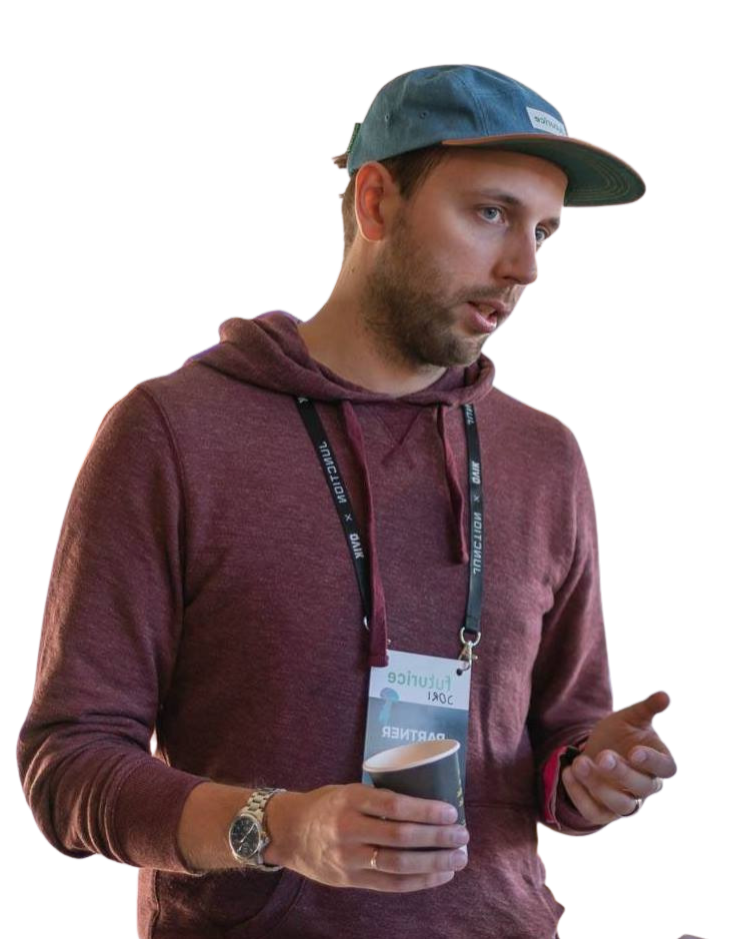
\includegraphics[width=23mm,clip,keepaspectratio]{jori.png} &   \textbf{Jori Mäkkeli}, DI, on jatko-opiskelija Aalto-yliopiston kauppakorkeakoulussa sekä työyhteisöjen kehittäjä digikonsultaatiotoimisto Futuricella. Jori kehittää ja haluaa ymmärtää paremmin yhteisöohjautuvia ja matalahierarkkisia organisaatioita. Hän tuo yhteisöohjautuvuutta ja työelämädemokratiaa työelämästä käytävään yhteiskunnalliseen keskusteluun ja työpaikkojen arkeen. \vspace{5mm}  \\

    
\includegraphics[width=20mm,keepaspectratio]{jp.png} &   \textbf{Jussi-Pekka Teini} edistää palkka- ja vapaaehtoistöissä kestävää teknologiayhteiskuntaa. Päivätöinään hän vie eteenpäin kestävää kehitystä TEKillä ja vapaa-ajallaan toimii Tieteen ja teknologian Vihreiden varapuheenjohtajana ja Vihreiden puoluehallituksessa. \vspace{5mm}  \\

    
\includegraphics[width=23mm,clip,keepaspectratio]{janne.png} &   \textbf{Janne Peltola} on yrittäjä, enkelisijoittaja/hallitusammattilainen ja perheenisä Tampereelta. Janne toimii Viitteen liittohallituksessa, Vihreiden puoluevaltuustossa sekä TEKin teknologiavaliokunnassa ja valtuustossa. Janne edistää kestävää kehitystä kaikilla sen osa-alueilla liiketoiminnalla ja laadukkaalla politiikalla.
\end{tabularx}

\chapter{Esipuhe - Työpahoinvoinnin pandemia}

\authorpic{janne}

Unohtakaa korona. Keskuudessamme vallitsee paljon laajempi, pirullisempi ja erikoisesti huomaamattomampi työpahoinvoinnin pandemia.

Erityisesti naisvaltaisilla aloilla tilanne on muuttunut hälyttävästi: puolet naistyöntekijöistä kärsivät väsymyksen ja tarmottomuuden tunteista ja heillä on myös vaikeuksia nukkua. Syy on työolobarometrin perusteella selkeä: vaikka 80 prosentilla työntekijöistä on mahdollisuuksia vaikuttaa työhönsä, naisista puolilla ei ole aikaa käsitellä uusia ajatuksia\sidenote{Mahdollisuuksien tasa-arvo ei voi toteutua, jos työelämässä ei ole uusille ajatuksille tilaa hautua ja hengittää.}. Kun otetaan huomioon miten työn merkityksellisyys ja mielekkyys muodostuvat suurelta osin juuri autonomian kautta, ei ole yllättävää että tästä seuraa voimattomuutta ja ahdistusta.

Mielenterveysperustaiset työkyvyttömyyseläkkeet ohittivat vuonna 2020 tuki- ja liikuntaelinten sairauksista johtuvat. Jokainen työkyvyttömyyseläke on, paitsi inhimillinen tragedia, myös tolkuttoman kallista yhteiskunnalle. Kuten edellä todettiin, hallinnan menettäminen ja epävarmuus ovat monen mielenterveysongelman juurisyy. Kiire ja epävarmuus ovat olleet prekariaatille tuttuja jo pitkään, mutta näiden ilmiöiden hiipiessä myös palkansaajien piiriin\sidenote{Prekariaatin - niin duunareiden kuin akateemistenkin - asema on ollut jo pitkään kehno. Sille pitäisi tehdä jotain, mutta olemme vielä merkittävämmän kestävyyskriisin äärellä jos sama ahdistus leviää palkansaajienkin puolelle.} olisi tarpeen alkaa katsoa peiliin ja miettiä, millaista työelämää haluamme rakentaa tulevaisuudessa ja millaisen työelämän jätämme tuleville sukupolville.

Pääoman vaatimukset työn tehokkuudelle ja yritysten tuottavuudelle ovat kasvaneet merkittävästi - pääasiassa koska pääoman omistajien vaatimukset pääoman tuottavuuden kasvulle ovat kasvaneet. Jokaisesta taseen eurosta on tiristettävä viimeisetkin tehot irti, jotta kapitalismi toimisi halutulla tavalla. Onko tämä se kapitalismi, jota haluamme\sidenote{Hyvä kapitalismi voisi korostaa myös sosiaalista ja ekologista pääomaa.}?

Tässä pamfletissa haluamme hahmotella vihreää työelämää, joka säilyttää kapitalismin parhaat puolet, mutta on samalla inhimillisempi, pitkäjänteisempi ja luovempi. Uskomme, että keskittymällä tehokkuuden sijaan työn laatuun voimme parantaa kaikkien suomalaisten oloja ja tehdä entistä parempaa tulosta. 

Otamme muutamia eri näkökulmia. Onko osakeyhtiö sittenkään paras tapa tehdä pitkäjänteistä liiketoimintaa? Onko feminismi sittenkin kilpailuetu? Miksi työpaikat edes tarvitsevat pomoja? Voisiko ekologisuus olla kilpailuetu myös henkilöstöpuolella? Miten työn kohtaanto ja algoritmisaatio kohdataan parhaalla mahdollisella tavalla?

Mikään työmarkkinajärjestö tai poliittinen puolue ei tällä hetkellä yritä ratkaista työpahoinvoinnin pandemiaa tosissaan. Uskomme, että näistä palikoista voidaan rakentaa, freesiä, vihreää työmarkkinapolitiikkaa 2020-luvulle ja siitä eteenpäin.

\tableofcontents

\part{12 teesiä parempaan työelämään}

\chapter{12 teesiä työelämästä}

\begin{description}
    \item[Työelämän hierarkkisuus on aiheuttanut työpahoinvoinnin pandemian.] Hallinnan tunteen katoaminen on aiheuttanut mielenterveysongelmien ja työkyvyttömyyden syöksykierteen. Hierarkioiden madaltaminen ja laadukas johtaminen poistaisi mielenterveysongelmia.
    \item[Työelämän laatu on tärkeämpää kuin pääoma.] Pääoma on yliarvostettua. Työ jalostaa pääoman uudeksi pääomaksi, joten työ on vähintään yhtä arvokasta kuin pääoma. Työtä pitää siis arvostaa yhtäläisesti, eli nykymuotoinen malli jossa pääoma tuottaa ikuiset osinkotulot mutta työ kertapalkan, pitää uudistaa.
    \item[Työ on yliarvostettua.] Täystyöllisyyden ja ikuisen 37,5 tunnin työviikon tavoitteluun jumiutunut yhteiskunta johtaa yhä laajenevaan työelämän hevonpaskaistumiseen sekä haitalliseen tuotantoon ja kulutukseen. Samalla ihmisten odotetaan käyttävän yhä suuremman osan vapaa-ajastaan osaamisen päivittämiseen ja työkyvyn ylläpitoon. Asetelma on muuttunut aivan perverssiksi.
    \item[Työelämä heikentää demokraattista yhteiskuntaa.] Nykyaikainen työelämä on harvainvallan päälle perustettu instituutio, joka rakentuu meritokratian illuusiolle. Nykyinen työelämä heikentää osallisuuden kokemusta ja opettaa, että päätökset yhteisistä asioista tekee joku muu. Montako epädemokraattista instituutiota aidosti demokraattinen yhteiskunta voi pitää sisällään?
    \item[Työelämä heikentää ihmisoikeuksia.] Nykyaikainen työelämä ei tue ihmisoikeuksien toteutumista. Nyt ihmisoikeuksistaan ja vapauksistaan saa luopua työsopimuksella. Millä perusteella vapaata ihmistä saa alistaa ja määrätä työelämässä?
    \item[Työelämä pilaa ilmaston ja luonnon.] Nykyaikaisen työelämän tehostuva toiminta tehostaa myös ympäristön rappeutumista. Niin kauan kuin kasvua ei saada irti kytkettyä ympäristöhaitasta, tehostuvan työelämän rakentama talouskasvu lisää ympäristön pahoinvointia. 
    \item[Työelämä ratkaisee vääriä ongelmia.] On helppoa tehdä paljon rahaa ja luoda kovaa uraa optimoiden somemainonnan algoritmeja tai tehostamalla öljynporausta pilvilaskennalla. On vaikeaa luoda uraa, jossa pelastaa maailma. Työelämän täytyy kehittyä niin, että viheliäisten ongelmien ratkaiseminen on liiketoiminnallisesti houkuttelevaa.
    \item[Työelämä tarvitsee intersektionaalista feminismiä.] Naisten ja vähemmistöjen osaamisen alihinnoittelu on räikeä todiste työmarkkinoiden epärationaalisuudesta. On aika jättää taakse tunne- ja ideologiaperustainen valkoista heteromiestä suosiva työelämä ja siirtyä rationaaliseen intersektionaaliseen feminismiin.
    \item[Intersektionaalinen feminismi tuo parhaat tuotot riistokapitalistille.] Naiset ja vähemmistöjen palkkatoiveet ovat matalampia kuin valkoisilla heteroinsinöörimiehillä, joten olisi epärationaalista olla palkkaamatta heitä. Kun rekrytoi ja johtaa intersektionaalinen feminismi edellä, on helpompi löytää juuri sopivat henkilöt edullisesti. Moninaisuuden kylkiäisenä saa kyvykkäämmän organisaation, riistokapitalistin rahasammon.
    \item[Työ on osa yhteiskuntaa ja siten osa politiikkaa.] Suomessa ollaan tuudittauduttu ajatukseen, että työelämän pelisäännöt ja kehittäminen voidaan jättää pelkästään työmarkkinajärjestöjen vastuulle. Työelämän laadulliset kysymykset on kuitenkin räikeästi laiminlyöty ja valtion täytyy tulla mukaan työelämän aktiiviseksi kehittäjäksi.
    \item[Kohta perinteinen organisaatio lentää roskiin ja sinäkin työskentelet algoritmille.]  Perinteinen organisaatio on olemassa lähinnä työn järjestelemistä varten. Pian työn voi kuitenkin optimoida digitaalisen alustan algoritmi, eikä organisaatioita enää tarvita. Alustan APIn yläpuolella olevat insinöörit määräävät, mitä APIn alla olevat alamaiset tekevät.
    \item[Maahanmuuttaja vaihtaa sinunkin vaippasi.] Pienenevät ikäluokat ja heikentyvä huoltosuhde luovat valtavan tarpeen työperäiselle maahanmuutolle. Saatavuusharkintaa ei tarvita, koska jokaisella alalla tulee olemaan työvoimapula. Jotta sinunkin vaippasi saadaan vielä joskus vaihdettua, pitää kaikki työperäisen maahanmuuton hidasteet poistaa heti.
\end{description}

\part{Mitä vihreän työmarkkinapolitiikan tulisi tavoitella?}

\chapter{Mitä haluamme työelämältä?}

Työelämä on surkealla tolalla, eikä se ole kehittymässä parempaan ilman merkittäviä toimenpiteitä ja paradigman muutoksia. Tarvitaan vihreää työmarkkinapolitiikkaa, joka rakentuu kestävän kehityksen periaatteille niin yksilö- kuin yhteiskuntatasolla. 

Oletamme talousjärjestelmän perustuvan ainakin vielä lähivuosikymmeninä kapitalistiseen markkinatalouteen, jossa kasvu on aina tavoiteltua.  Vaikka sen hegemoniaa ei ole lähdetty tässä pamfletissa haastamaan, on syytä jatkaa paremman järjestelmän etsimistä. Tarjoaako tuunattu kapitalistinen markkinatalous tai jokin muu järjestelmä kokonaisratkaisun, jossa työelämä ei ole enää synonyymi ympäristön ja ihmismielen tuhoamiselle? Olemme avoimia kaikille vaatimuksemme täyttäville vaihtoehdoille, oli se sitten kapitalistisen markkinatalouden korjaaminen tai täysin uusi talousjärjestelmä. 

Kaikesta ansaitusta kritiikistä huolimatta huolimatta kapitalistinen markkinatalous on tähän asti esitetyistä malleista tehokkain tapa järjestää talous. Donitsitalous ei vastaa kysymykseen siitä, miten seitsemän miljardia ihmistä saadaan vetämään yhtä köyttä, eikä degrowth vastaa kunnolla siihen, miten väistämätöntä kurjuutta jaetaan sosiaalisesti oikeudenmukaisesti. Me katsomme, että markkinatalous on paras tapa jakaa niukkoja resursseja, kunhan järjestelmä kalibroidaan oikein.

Silti on selvää, että nykytila ja nykyinen kehityssuunta ei ole vaihtoehto. Työpahoinvoinnin pandemia, ympäristökriisit, vallan ja varallisuuden keskittyminen ja lukuisat muut haitalliset kehityskulut on saatava kuriin. Tässä luvussa hahmottelemme miltä tulevaisuuden kestävä työelämä näyttää niin yksilön kuin eri yhteiskunnallisten ulottuvuuksien kautta. 

\chapter{Yksilölle merkityksellinen ja kestävä työ }
\authorpic{jori}

Työelämä ei ole irrallinen osa yhteiskuntaa vaan olennainen osa
aikuisväestön ajan- ja energiankäyttöä. Se on myös merkittävimpiä
tapoja, jolla yksilö osallistuu yhteiskunnan toimintojen ylläpitoon ja
kehittämiseen. Työelämällä ja sen laadukkuudella on siis yksilön
kannalta suuri merkitys. On olennaista\sidenote{Työn on oltava yksilön kannalta merkityksellistä ja kestävää sekä ihmisarvoa tukevaa.}, että työ on yksilön kannalta
merkityksellistä ja kestävää sekä ihmisarvoa tukevaa.

Tiivistetysti ihmisarvoinen työ takaa minimissään ihmisten ruumiillisen,
henkisen ja sosiaalisen turvallisuuden ja koskemattomuuden. Käytännössä
tämä tarkoittaa työsuojelua, joka käsittää sekä fyysisen että henkisen
turvallisuuden työyhteisöissä ja itse työtä tehdessä\sidenote{Työsuojelu keskittyy usein ns. hygieniatekijöihin, eli niihin asioihin jotka varmistavat työympäristölle tietyn minimitason.}. Lisäksi
työsuojelun tulee ottaa huomioon se sosiaalinen ympäristö, jossa työtä
tehdään. Jos asiakkaat tai kollegat kohtelevat epäasiallisesti (ollen
esimerkiksi syrjiviä, rasistisia tai seksistisiä), tulee siihen puuttua
työsuojelun puitteissa. Aikamme erityspiirteenä työsuojelussa on
ihmisten suojaaminen kiireeltä ja mielenterveyden ongelmilta
työelämässä. Jatkuva tehostamisen ideologia on johtanut siihen, että
työelämän vaativuus ja tempo ovat kasvaneet ja samaan aikaan erilaisia
tukiresursseja ja avustavia työrooleja on karsittu. Lisäksi myös
työelämän ulkopuoliset vaatimukset ovat lisääntyneet (esimerkiksi
kuluttajana, harrastajana tai vanhempana) ja yhä useammin työ tunkeutuu
osaksi vapaa-aikaa. Näiden seurauksena jaksamisongelmat ovat yleistyneet
työelämässä ja ovat erityisesti esillä nuorilla aikuisilla ja naisilla
(Sutela, 2020).

Työsuojelun tavoite ei ole ainoastaan käsitellä ja ratkaista jo olemassa
olevia ongelmia, vaan myös ennaltaehkäistä niitä ja aktiivisesti tukea
ihmisten fyysistä ja henkistä hyvinvointia työpaikoilla\sidenote{Hygieniatekijöiden lisäksi tulisi tarkastella huolellisesti myös motivaattoreita, eli niitä tekijöitä jotka saavat ihmisen viihtymään ja kukoistamaan.}. Uuden
aikakauden työsuojelun tulee olla myös proaktiivista ja aktiivisesti
hyvinvointia tukevaa (ns. positiivista työsuojelua). Tutkimusten mukaan
ihmisten keskeisiä psykologisia perustarpeita ovat omaehtoisuuden,
kyvykkyyden ja yhteenkuuluvuuden kokemukset (Ryan \& Deci, 2000). Näiden
täyttyminen (subjektiivisessa, ei objektiivisessa mielessä) tuottaa
hyvinvointia. Kehittämällä työtä, työpaikkoja ja työelämää suuntaan,
joka tukee näitä kolmea perustarvetta, on mahdollista korjata ja
ehkäistä pahoinvointia sekä lisätä työelämän tuottamaa henkistä
hyvinvointia yksilölle.

\textbf{Omaehtoisuuden }\sidenote{Modernin työpaikan on tuettava omaehtoisuuden, kyvykkyyden ja yhteenkuuluvuuden kokemuksia.} kokemuksen tukeminen työpaikoilla tarkoittaa
yksilön kykyä vaikuttaa siihen, mitä työtä tehdään, miten sitä tehdään
ja miksi työtä tehdään. Kyky vaikuttaa ei tarkoita sitä, että jokainen
saisi päättää nämä kaikki osa-alueet itsenäisesti, vaan tärkeintä on
aito vaikuttamisen mahdollisuus. Päätöksiä voidaan tehdä yhdessä tai
hierarkkisesti, mutta joka tapauksessa jollakin tavalla osallistavasti
tai yhteisesti. \textbf{Kyvykkyyden }kokemuksen tukeminen työpaikoilla
tarkoittaa työnkuvien ja tehtävien muokkaamista siihen suuntaan, että
niistä on mahdollista selviytyä nykyisellä osaamisella tai osaamista
kehittämällä. Tämä ei tarkoita, että työn haastavuutta tai tavoitteita
ei saisi nostaa. On kuitenkin huolehdittava siitä, että työntekijöillä
on mahdollisuus toimia osaamisensa rajojen sisällä tai aivan niiden
läheisyydessä flow-tilan mahdollistamiseksi ja oppimisen tukemiseksi.
Kaiken työn ei kuitenkaan tarvitse olla (tai saakaan olla) jatkuvasti
haastavaa. \textbf{Yhteenkuuluvuuden }kokemuksen tukeminen työpaikoilla
tarkoittaa mahdollisuutta muodostaa lähipiiri ja jonkinlainen tiivis
työyhteisö, johon ihminen kokee kuuluvansa. Työyhteisön ei kuitenkaan
tarvitse kilpailla ihmisten muiden lähiyhteisöjen kanssa. Täytyy olla
myös sallittua ``käydä vain töissä''ja olla kiinnittymättä vankasti
työyhteisöön.

Hyvä ja ihmisarvoa tukeva työelämä on keskeinen osa hyvin toimivaa ja
kestävää yhteiskuntaa. Kehittämällä työtä, työpaikkoja ja työelämää
työntekijöiden hyvinvointia aktiivisesti tukevaan\sidenote{Työpaikkojen on mietittävä uudestaan, missä kulkevat hygienia- ja motivaatiotekijöiden rajat. Hyvinvointi ei ole bonus, vaan oleellinen osa hyvää työtä.} suuntaan voidaan
tavoitella työelämää, joka edistää ihmisten psykososiaalisten ja
fyysisten tarpeiden täyttymistä osana työn tekemisen arkea. Samalla se
takaa ihmisarvon (esimerkiksi vapaus, yhdenvertaisuus, arvokkuus,
fyysinen koskemattomuus, uskonnon ja ajattelun vapaus) toteutumisen myös
työelämässä.

\chapter{Sosiaalisesti kestävä työ }
\authorpic{janne}

Työ käsitetään usein taloudellisena instituutiona, mutta sillä on myös
merkittäviä sosiaalisia ulottuvuuksia. Työ on tapa kiinnittyä
yhteiskuntaan, se muodostaa monille tärkeän sosiaalisen ja inhimillisen
verkoston ja toisaalta - kuten sosiaaliturvan
vastikkeellisuuskeskustelusta voidaan nähdä - monille työ on itseisarvo
ja tapa saada osakseen yhteiskunnan turva.

Kaikilla ei kuitenkaan ole realistista mahdollisuutta tehdä työtä - tai
ainakaan sellaista työtä joka koetaan yleisesti taloudellisesti
hyväksyttäväksi.\sidenote{Meidän on laajennettava sosiaalisesti hyväksytyn työn ikkunaa niin, että kaikki yhteiskuntaa ylläpitävä työ koetaan arvokkaaksi.} Hoivatyötä tekevät omaishoitajat ja kotivanhemmat,
tunnetyötä tekevät perheiden ja työyhteisöjen hiljaiset sankarit,
aktivistit tai vaikkapa vapaaehtoisesti internetin kulmakiviä
kannattelevat avoimen lähdekoodin ohjelmoijat jäävät helposti tässä
arvokäsityksessä paitsioon.

Samaten paitsioon jäävät työmarkkinoilla sorsitut ihmisryhmät.\sidenote{Moni on työmarkkinoilla osaton vailla omaa syytään. Siksikin sosiaalisen arvon sitominen työhön on vaarallista.} Kun
suomalaisista työnantajista vain joka neljäs suostuu palkkaamaan
työntekijän jolla ei ole sujuvaa suomen kielen taitoa, perhehaaveista
kysellään yhäkin työhaastatteluissa, romanin on parasta hakea töitä
kantasuomalaisella nimellä ja opot ohjaavat somalitytöt lähihoitajiksi,
ei pidä ihmetellä miksi yhteiskunta segregoituu.

Täystyöllisyys on osa yhteiskuntamme sosiaalista sopimusta, jossa
vapaamatkustajia katsotaan pahalla ja kaikkien oletetaan pyrkivän
työllistämään itsensä nopeasti työttömyyden sattuessa omalle kohdalle.
Tämä sosiaalinen sopimus osaltaan synnyttää myös tyhjänpäiväisiä
työpaikkoja kun työpaikkojen kadotessa keksitään uusia.\sidenote{Työn määrä kasvaa täyttämään 37,5-tuntisen tilan, vaikka se ei olisi tarpeen.} Ekonomisti John
Maynard Keynes arvioi vuonna 1930, että hänen lapsenlapsensa tekisivät
15-tuntista työviikkoa, kun teknologia automatisoisi työtä. Keynes oli
väärässä, ja antropologi David Graeber selittää tämän matalan
tuottavuuden sontatyöllä (\emph{bullshit job}), joka syntyy tilaan josta
vanha työ katoaa.

Sontatyö on sosiaalinen välttämättömyys yhteisössä, jossa yksilön arvo
ja identiteetti syntyvät työn kautta. Mahdollisimman korkeaan
työllisyyteen nojaava yhteiskuntamme on viritetty arvostamaan kaikkea
perinteistä työtä.\sidenote{Koska materiaalinen kulutus ja talouskasvu ovat erottamattomasti kytkeytyneet toisiinsa, meillä ei ole enää varaa perinteiseen työkäsitykseen.} Tähän luksukseen meillä ei ole enää ekologisesti varaa, koska
jatkuvaa talouskasvua ei ole saatu irrotettua materiaalisen kulutuksen
kasvusta. On siis ekologisesti vastuullista pohtia tarkemmin, mikä
yhteys työn yhteiskunnallisella merkityksellä ja kestävällä kehityksellä
on.

Jos työ ei enää olisikaan yhteiskunnallisen osallisuuden kulmakivi, mitä
tapahtuisi? Globaalisti kilpaillussa markkinataloudessa yksittäisen maan
on vaarallista leppoistaa talouttaan liikaa: korkean tuottavuuden työ
karkaa ulkomaille ja vaihtotase notkahtaa vaarallisesti.\sidenote{Työelämän leppoistaminen yksin kilpaillussa globaalissa markkinataloudessa on vaarallista.} Polkuriippuvuus
on pirullinen. Ei ole myöskään täysin selvää, miten esimerkiksi
perustuloon pohjautuva turvaverkko ja avoin maahanmuuttopolitiikka
nivoutuvat järkevästi yhteen.

Tästä huolimatta - ja juuri tämän vuoksi - on avattava keskustelu
sosiaalisesti kestävästä työstä. Työ ei saa määrittää ihmistä, tai
sitten meidän pitää määritellä työ uudestaan siten, että useampi voi
kokea kuuluvansa osaksi yhteiskuntaa joka sitä niin kovasti arvostaa.

\chapter{Ekologisesti kestävä työ }
\authorpic{jp}

Kuolleella planeetalla ei ole työpaikkoja. Toteamuksella on monta
merkitystä: toisaalta se tarkoittaa, että työmarkkinatoimijat eivät enää
voi sivuuttaa ilmastokriisiä omassa toiminnassaan, ja toisaalta että
työmarkkinapolitiikka tulee huomioida osana ilmastopolitiikkaa.

Kansainvälinen ay-liike on puhunut jo pitkään oikeudenmukaisesta
siirtymästä (just transition). Ilmastotoimien oikeudenmukaisuus on
sittemmin saanut muitakin vakiintuvia merkityksiä, mutta alunperin
oikeudenmukainen siirtymä on koskenut nimenomaan työmarkkinakysymyksiä:
miten siirtymä ilmastoystävälliseen yhteiskuntaan tehdään niin, että
ilmastotoimien vuoksi työpaikkansa menettävät löytävät uutta mielekästä
työtä? \sidenote{Miten muutamme työntekijät autettavista objekteista aktiivisiksi oman, uuden vihreän elämänsä luojiksi?} Tämä on ollut myös toistaiseksi vallitseva työelämäkysymys
kestävästä siirtymästä puhuttaessa, vaikka aihe ansaitsisi paljon
laajempaa tarkastelua. Oikeudenmukainen siirtymä tarkastelee, miten
yhteiskunta tukee työntekijöitä murroksessa. Yhtä tärkeää olisi miettiä,
miten työntekijöille saataisiin valtaa ottaa aktiivista toimijuutta
työmarkkinoiden ympäristöystävällisyyden edistämiseksi.

Tulevaisuudessa jokaisen työpaikan on oltava ilmastopositiivinen tai
vähintään -neutraali. Vaikka ympäristön kannalta positiivisen tai
vähintään neutraalin työn määrittely on äärimmäisen vaikeaa, siihen on
silti pyrittävä. Kun kyseessä on ympäristövaatimusten minimitason
määrittely, on regulaatio paras työkalu sen edistämiseen. Tämä työ on jo
hyvällä alulla niin Suomessa kuin EU:ssa esimerkiksi päästökaupan ja
kiertotaloussäätelyn myötä.

Toisekseen työntekijöille tulisi saada neuvotteluvaltaa ympäristölle
haitallisesta työstä kieltäytymiseksi\sidenote{Työntekijöille tulisi saada neuvotteluvaltaa ympäristölle
haitallisesta työstä kieltäytymiseksi}, jolloin ympäristölle
haitallisesta työstä täytyisi maksaa enemmän palkkaa ja sen teettäminen
olisi vähemmän kannattavaa. Kun oman työuran ympäristöystävällisyys
olisi omissa käsissä, yhä useampi voisi tehdä arvojensa mukaista työtä.

Ekologisesti kestävää työtä on tarkasteltava myös isommassa kuvassa.
Elämme aikaa, jolloin yhteiskunnan aitoja suuria ongelmia, kuten nälkää,
janoa, köyhyyttä, yksinäisyyttä, hoivaa tai ilmastonmuutoksen
pysäyttämistä ei ole liiketoiminnallisesti houkuttelevaa ratkaista eikä
näiden ympärille synny merkittävää määrää työtä. Sen sijaan työllä
tuotetaan valtava määrä turhaa kulutusta, kuten suuri osa kaikesta
kuluttajille suunnatusta teollisesta ja ohjelmistotuotannosta, tai
pelkkää kuumaa ilmaa kuten suuri osa finanssialaa.

Työ on iso osa identiteettiä ja kestävyysmurroksen myötä monien
identiteetti on murroksessa. Muutos voi olla merkittävä esimerkiksi
kiertotalouden edetessä, kun yhä harvemman työssä valmistetaan uusia
tuotteita ja vastaavasti yhä useamman työ on vanhaa korjaavaa ja
ylläpitävää. \sidenote{Kiertotalous tulee muuttamaan merkittävästi myös työn luonnetta.}
Lineaaritalouden rakenteisiin varttuneille ja
ehdollistuneille tämä identiteetin muutos voi tuntua ikävältä ja
taantuvalta sen sijaan, että se nähtäisiin innostavana ja arvokasta
säilyttävänä. Yhteiskunnan normien ja arvojen tulisikin muuttua
etupainotteisesti suhteessa työhön, jotta työn kestävyysmurros olisi
kokemuksena voittopuolisesti myönteinen.

Ympäristöystävällisen tai minimissään ympäristöneutraalin työn tulee
olla mahdollisimman pian kaikkien perusoikeus. Työn
ympäristöystävällisyydelle täytyy luoda nykyistä työturvallisuutta
vastaava vaatimustaso, jonka jokaisen työpaikan on minimissään
täytettävä. Työntekijöiden omaa valtaa ohjata työuraansa
ympäristöystävällisempään suuntaan on tuettava antamalla asiassa
työntekijöille valtaa muodossa tai toisessa. Konkreettisesti tavoitetta
voisi edistää esimerkiksi taloudellista turvaa tuovalla perustulolla
sekä luomalla työpaikoille ympäristövaltuutetun roolin.

\chapter{Taloudellisesti kestävät työn rakenteet }
\authorpic{jp}

YK:n kestävän kehityksen tavoitteet huomioivat talouden erityisesti
neljän tavoitteen kautta: säällinen työ ja talouskasvu; teollisuus,
innovaatiot ja infrastruktuuri; eriarvoisuuden vähentäminen; sekä
vastuullinen kulutus ja tuotanto. On huomionarvoista, että talouden
kasvuhakuisuus on sisäänleivottuna myös näihin tavoitteisiin. Vaikka
nykyisin keskustelu degrowth-ajattelun ympärillä on yhä vilkkaampaa, on
kasvun tavoittelun hegemonia vielä toistaiseksi kiistaton.
Degrowth-liikkeen edistämä keskustelu ikuisen kasvun tavoittelun
ilmeisistä haitoista on kuitenkin tarpeellista, mutta vielä toistaiseksi
se ei ole onnistunut tarjoamaan vastauksia miten ei-kasvuhakuinen
talousjärjestelmä olisi taloudellisesti kestävä. Kun koko yhteiskuntaa
on vuosikymmeniä rakennettu kasvun varaan valtioiden taloutta isompia
eläkejärjestelmiä myöten, ei irtautumista kasvun tavoittelusta voi
ohittaa olankohautuksella.

 Kasvavan talouden aikaan \sidenote{Talouskasvulla on ilmeiset etunsa.} ihmiset ovat
tyytyväisempiä joka mahdollistaa myös kunnianhimoiset ympäristötoimet.
Kasvua voidaan ohjata tukemaan kestävyystavoitteita ohjaamalla taloutta
kohti tarvittavia ratkaisuja ja pois ei-toivotuista. Kasvu myös takaa
että tarvittaviin kestävyysmurroksen investointeihin löytyy paremmin
rahoitusta.

Kasvulla on kuitenkin rajansa eikä talousjärjestelmää voi rakentaa
loputtomiin sen varaan. Kasvuhakuisuudesta luopuminen olisi myös
ympäristöllisen kestävyyden kannalta toivottavaa, erityisesti koska on
epäselvää voiko talouskasvun absoluuttista irtikytkentää
ympäristöhaitoista koskaan tapahtua. \sidenote{Absoluuttinen materiaalisen kulutuksen ja talouskasvun irtikytkentä ei ole tapahtunut, ja tuskin tapahtuu.} Kasvuriippuvuudesta irtautumista
onkin syytä tutkia aktiivisesti ja etsiä mahdollisuuksia
toteuttamiskelpoiseen irtautumiseen ja uuteen järjestelmään.
Kasvuriippuvuus on kuitenkin yhteiskunnan rakenteissa niin syvällä,
ettei tämän voi odottaa tapahtuvan nopeasti vaan aikaisintaan
vuosikymmenten aikajänteellä. Siksi on samaan aikaan edistettävä
nykyisen kasvuhakuisen kapitalistisen markkinatalousyhteiskunnan
kehittämistä planetaarisia rajoja ja ihmisten hyvinvointia
kunnioittavaksi.

Kasvuriippuvuutta haastaa myös talouskasvun hidastuminen. Talouskasvu
rakentuu kahdesta osasta: väestön kasvusta ja tuottavuuden kasvusta.
Rikkaissa maissa, ja vuosikymmenten aikajänteella koko maailmassa,
väestön määrä on kääntymässä laskusuuntaan.\sidenote{Talouskasvu heikkenee tulevaisuudessa joka tapauksessa, mikä tekee kasvuriippuvuudesta irtautumisesta entistäkin ajankohtaisempaa.} Kun tähän trendiin yhdistää
esimerkiksi työmarkkinoiden palveluvaltaistumisen ja
hevonpaskaistumisen, on kasvun suhteen joka tapauksessa tiedossa
vaikeita aikoja pitkällä tähtäimellä.

Degrowth-liikkeellä on jaloja tavoitteita, jotka ovat kannatettavia
riippumatta talousjärjestelmästä. \sidenote{Degrowth-liikkeellä on jaloja tavoitteita, jotka ovat kannatettavia
riippumatta talousjärjestelmästä.} Takuutyöllisyys, työelämän
demokratisaatio, kerskakuluttamisen lopettaminen ja varallisuuserojen
kaventaminen ovat tarpeellisia tai vähintään harkinnan arvoisia
tavoitteita myös kapitalistisessa markkinataloudessa.

Optimaalinen talousjärjestelmä tuottaisi meille säällisen elintason ja
samaan aikaan parantaisi luonnon tilaa ja ihmisten hyvinvointia. Se
ohjaisi talouden toimijat ratkaisemaan oikeita, viheliäisiä ongelmia eli
esimerkiksi nälkää ja köyhyyttä sen sijaan, että se tuottaa valheellista
hyvinvointia teettämällä työtä, jolla on olevinaan tarkoitus ja
kulutusta, joka on tuottavinaan onnellisuutta.

\part{Haasteet}

\chapter{Mikä työelämässä on pielessä?}

Nykytyöelämässä riittää haasteita ja haitallisia kehityskulkuja.
Ongelmiin on puututtava ajoissa ennen ongelmien kärjistymistä
kriiseiksi.

Epätyypillisistä työsuhteista alkaa tulla niin yleisiä, että
kehityksen jatkuessa epätyypillisistä työsuhteista on tulossa normi.
Varallisuuserot uhkaavat revetä kuiluksi eri ihmisryhmien
välillä koska pääomaa kohdellaan yhteiskunnassa työtä arvokkaampana
tekijänä. Työmarkkinoiden kohtaanto-ongelmat aiheuttavat haasteita niin
työnhakijoille kuin työvoimaa etsiville, kun kummankaan toiveet eivät
täyty. Työmarkkinatoimijat ovat
jumittuneet riitelemään pelkistä palkoista eikä työelämän laadullinen
kehittäminen ole kenenkään käsissä. Maahanmuuttajat, niin matalasti kuin
korkeasti koulutetut, joutuvat kohtaamaan Suomen kahdet työmarkkinat,
joissa heille jää luu käteen.

Työelämän hierarkioista pidetään kiinni hampaat irvessä, vaikka
niistä joustaminen voisi edistää laajasti työntekijöiden hyvinvointia ja
tukea yhteiskunnan instituutioiden myönteistä kehittymistä.
Työpahoinvoinnin pandemia uhkaa pahentaa surkealla tolalla olevaa
huoltosuhdetta edelleen, ja mielenterveyden ja jaksamisen haasteiden
yksilötason tragediaa ei sovi sitäkään sivuuttaa. Työn ekologiset
vaikutukset ovat järjestelmällisesti haitallisia, eikä muutos parempaan
tapahdu läheskään tarvittavalla nopeudella. 

Tunnistettujen ja käsiteltyjen haasteiden lista ei ole kattava, vaan
pakostakin heijastaa pamfletin tekijöiden omaan työelämäkokemukseen
liittyviä havaintoja. Mutta kyllä tässäkin pohdittavaa riittää.

\chapter{Epätyypilliset työsuhteet ja työn muotojen polarisaatio }
\authorpic{jori}

Epätyypillisillä työsuhteilla (tai epätyypillisellä työllä) tarkoitetaan
sellaisia työsuhteita, jotka ovat osa-aikaisia, määräaikaisia tai näiden
yhdistelmä. Lisäksi joskus mukaan lasketaan myös työsuhteet, jotka ovat
jatkuvasti kilpailutuksen kohteena (esimerkiksi työpaikka on sidottu
asiakkuuden jatkumiseen ja että tätä kautta irtisanomisen uhka on
jatkuva). Vuonna 2018 15-64 vuotiaista työllisistä 24 \% oli erilaisissa
epätyypillisissä töissä ja 6 \% työllisti itsensä yrityksen tai
toiminimen kautta (Ojala, 2020). Jos noin 30\% työvoimasta on
epätyypillisissä työsuhteissa, onko se enää epätyypillistä?\sidenote{Jos kolmannes työvoimasta on epätyypillisessä työssä, on kyse jo varsin tyypillisestä toiminnasta.} Ongelmaa
epätyypillisessä työssä ei ole, mikäli se on vapaaehtoista. Kuitenkin
näyttää siltä, että tästä 30 \%:stä puolet eli 15 \% on
vastentahtoisesti tällaisessa työsuhteessa. Lisäksi 19 \% yrittäjistä on
vastentahtoisesti yrittäjiä (Ojala, 2020).

Eräästä näkökulmasta epätyypillisen työn lisääntymisen ajatellaan olevan
hyvä asia, koska se lisää työvoiman joustoa. Suomen työmarkkinoita
pidetään jäykkinä. Todellisuudessa Suomessa ovat jäykkää lähinnä
palkanmuodostus ja ei-tuotantannollistaloudellinen irtisanominen. Suomen
työmarkkinat ovat itseasiassa varsin joustavat, jos tarkasteluksi
otetaankin työajat, irtisanomisen helppous tuotannollistaloudellisista
syistä, töiden ulkoistaminen määräaikaisille alihankkijoille tai
sopimusmuotojen määrääminen (määräaikaisketjutukset, osatyösopimukset
jne.). \sidenote{Monet Suomen työmarkkinoiden piirteet ovat itse asiassa paljon joustavampi kuin julkisesta keskustelusta arvaisi.}Ottaen huomioon tämän lisäksi, että noin 30 \% työstä on
joustavaa/epätyypillistä työtä, on hyvä kyseenalaistaa ovatko Suomen
työmarkkinat todella niin jäykät kuin väitetään.

Lisääntyneen ja vakiintuneen epätyypillisen työn lisäksi työelämään
vaikuttaa myös työn polarisaatio.\sidenote{Työn intensiivisyys jakautuu epätasaisesti, mikä on itsessään rakenteellinen ongelma työelämässä.} Tilastokeskuksen analyysissä lähes
puolta työssäkävijöistä vaivaa liian korkea työn intensiivisyys, joka
syö hyvinvointia (Sutela, 2020). Lisäksi kuormittavat työt ja
suorittavat rankat työt keskittyvät enemmän naisille (26\% miehillä -
35\% naisilla). Sukupuolen lisäksi huomiota herättää koulutusasteen
vaikutus työn luonteeseen. Kiireen pilaamat työt keskittyvät erityisesti
korkeakoulututkinnon suorittaneille (72\%) ja myös kuormittavissa töissä
korkeakoulutettujen osuus on suuri (66\%). Sen sijaan suorittavat rankat
työt keskittyvät vain toisen asteen koulutuksen suorittaneille.

Kyse on siis sekä sukupuoli- että koulutusasteasiasta.\sidenote{On ensisijaisen tärkeää lähteä korjaamaan näitä sukupuolten ja koulutusasteiden välisiä hyvinvointikuiluja.} Naisvaltaisten
töiden kiire ja intensiivisyys täytyy ottaa prioriteetiksi työoloja
parannettaessa ja palkkausta kehitettäessä. Edunvalvontatyötä tarvitaan
sekä kiireen vähentämiseksi asiantuntijatöissä ja korkeasti
koulutetuilla aloilla, että työn inhimillistämistä matalamman
koulutusasteen suorittavilla töille.

Yhteiskuntamme pitää ottaa paremmin huomioon
``epätyypilliset''työsuhteet, sillä ne ovat yleisiä ja sosiaaliturvan
rakentaminen täysipäiväisen työsuhteen oletukselle on vakava puute monen
suomalaisen näkökulmasta. Samalla kansalaiselle pitää antaa
subjektiivinen oikeus lyhyempään työaikaan. Epätyypillisten töiden
osalta tavoite tulee olla, että vastentahtoisesti tällaisessa töissä
olevien määrä saataisiin vähenemään.

\chapter{Tulojen ja varallisuuden jaon logiikka }
\authorpic{janne}

Vasemmistolainen talouskeskustelu sai uutta virtaa Pikettyn \emph{Pääoma
2000-luvulla }-raamatun julkaisusta. Havainto, että pääoma tuottaa
pitkällä aikavälillä työtä enemmän oli ansiokkaasti tilastoaineistolla
perusteltu ja johtopäätös varallisuuden kasautumisesta on todellinen
uhka. Pikettyä lukiessa on luonnollisesti pidettävä mielessä esimerkiksi
Gregory Mankiwin ansiokas kritiikki, jossa osoitetaan useiden jo
olemassa olevien yhteiskunnallisten rakenteiden suitsivan tehokkaasti
dynastioiden syntyä.\sidenote{Piketty on sekä oikeassa että väärässä, ja tulonjakokeskustelu aivan kummallisilla raiteilla. } Siksi seuraavassa keskitytään tulonjaon vähemmän
puhuttuun puoleen: korkeasti tuottavien ammattien motivaatiotekijöihin
ja niiden yhteyteen tulonjakoon.

Motivaation lisäksi tulojen ja varallisuuden muodostumisperusteet ovat
myös olennaisia yhteiskunnan turvaverkkojen toimintalogiikan kannalta.
Kiinteät, elinkustannuksiin sidotut palkat ovat merkittävä tekijä siinä,
miksi makrotaloudessa nähdään liiketoimintasyklejä. Jos palkat ja
ostovoima joustaisivat tehokkaammin ajassa, voitaisiin suhdannevaihtelua
keventää merkittävästi. Naiivisti voisi ajatella, että
pääomapainotteisempi palkitseminen olisi helppo ratkaisu.\sidenote{Onko palkkaperustainen palkitseminen ylipäätään makrotaloudellisesti paras ratkaisu?} Käytännössä
kuitenkin pääomapalkitseminen palkitsee ylikorostuneesti niitä, joilla
pääomaa on vanhastaan, sillä veroseuraamukset, pääoman hallinnan
kustannukset ja huonoista valinnoista seuraava urapalkkakehityksen
\emph{opportunity cost }ovat pienituloisille suuria. Onko siis
löydettävissä palkitsemismalli, joka ei lankea tähän ansaan?

Teollisen yhteiskunnan logiikka oli hyvin yksinkertainen: rakennetaan
tehdas, palkataan henkilökunta ja osoitetaan heille paikka koneistossa
ja tuotetaan hyödykkeitä niin että marginaalikustannus on
marginaalituoton verran. Jos tuotto ei ollut riittävää, voitiin
optimoida prosesseja.\sidenote{Teollisissa prosesseissa tuotannon tekijät olivat usein keskenään vaihdannaisia, jolloin pääoma määritti menestystä.} Tällaisessa ympäristössä oli luontevaa, että
pääoma myös palkitaan tuloksesta: tuottoa ei olisi olemassa ilman
tehdasta ja työvoimaa kannattaa kompensoida suoritteesta.

Modernissa tietotyöhön keskittyvässä yrityksessä seinät eivät enää
olekaan yhtä tärkeitä. Nyt suurin osa yrityksen arvonlisästä syntyy
tekijöiden osaamisen jalostamisesta tuotteeksi, joka kohtaa markkinoiden
tarpeet ja luo arvoa. Osaajien palkat eivät kuitenkaan ole halpoja:
tuotteen kehittäminen maksaa paljon, koska parhaat osaajat myös haluavat
parasta palkkaa. Samaten tuotteen markkinointi erityisesti
kuluttajamarkkinoilla on kallista: Applen sovelluskaupassa top-10:een
nouseminen on miljoonainvestointi, eikä takaa vielä mitään pysymisestä
listoilla.\sidenote{Rahalla ja investoinneilla on yhä väliä, mutta enenevissä määrin työn (eli sen tekijöiden) laadulla on enemmän väliä. Työ jalostaa pääoman uudeksi pääomaksi.} On kuitenkin selvää, että työn arvo on noussut vähintään
pääomaan rinnasteiseksi: kumpaakin tarvitaan, jotta voidaan rakentaa
kestävää ja kannattavaa liiketoimintaa.

Eikö korkea palkka ole riittävä palkkio tuottavuudesta? Työn hinta
muodostuu markkinoilla, eikä ole suoraan sidoksissa yksilön
tuottavuuteen. Työehtosopimusjärjestelmä ankkuroi palkkojen alapään, mutta mitä yksilöllisempi osaaminen yksilöllä on, sitä
yrittäjämäisemmin hän voi ulosmitata tämän osaamisen tuottaman
arvonlisän yritykselle, mutta tämä voi tapahtua vasta kun arvo on
osoitettu.\sidenote{Palkat muodostuvat markkinoilla, eivätkä tehdyn työn arvonlisästä. Pääoman palkkio taas muodostuu markkinoilla.} Kasvuyrityksen alkuvaiheissa ei ole varaa maksaa
markkinapalkkoja, mutta tästä kompensoidaan tyypillisesti potilla
pääomaa, jota usein luovutetaan tipoittain ajan yli sitouttamiskeinona.
Tämä on toisaalta fiksua, mutta toisaalta pääoman ehdoilla tapahtuvaa
palkitsemista.

Osakeyhtiöjärjestelmä syntyi mahdollistamaan kolonialistisen
maustekaupan, jossa pääoma otti riskiä varustamalla laivoja. Tämä oli
riskialtis, puhtaasti pääomavetoinen toiminta jossa varhain mukaan
tullut pääoman tarjoaja sai pysyviä tuottoja pääomalleen osakkeen
kautta. Ei ole selvää, että tämä järjestelmä on enää tietotyön
ympäristössä täysin validi.

Oikeudenmukaisempaa yksilölle olisi saada sitä suurempi osuus yrityksen
tuotoista mitä enemmän hän on sille tuottanut. Osuuskuntajärjestelmässä
pääoma (eli osakkeiden myynti) katsotaan velaksi, jota maksetaan
takaisin korkojen kera, mutta osallistuminen (eli osuuksien ostaminen ja
palveluiden käyttäminen) katsotaan toiminnaksi, joka oikeuttaa osuuteen
osuuskunnan ylijäämästä (eli voitosta).\sidenote{Osuuskuntajärjestelmässä on luotu erilainen yritystalouden kulttuuri, jossa tase on tuloslaskelmaa tärkeämpää ja työpanoksesta palkitaan.} Työosuuskunnassa siis eniten
töitä tehnyt saa suurimman osuuden ylijäämästä ja pääoman tarjoajan
panosta maksetaan takaisin kun liiketoiminta sen sallii.

Ei ole kohtuutonta sanoa, että osuuskunta-ajattelu lyö yli toiseen
suuntaan: pääoma ottaa riskiä, ja sitä vastaan on kohtuullista odottaa
kiinteää korkoa parempaa palautusta. Mutta onko riski riittävä oikeutus
rajattomaan tuottokattoon?\sidenote{Mikä oikeuttaa osakkeenomistajan ikuisen oikeuden osinkoon kertasuoritteesta?} Onko pääoma niin välttämätöntä, että siitä
tulee saada pysyvä osuus yrityksen tuotosta? Toisaalta: tuleeko minkään
oikeuttaa pysyvään osuuteen liiketoiminnan tuotoista?

Piketty perustelee kirjassaan Capital in the 21st Century laajalla
tilastoaineistolla käsitystään, että pääoma tuottaa systemaattisesti
paremmin kuin työ. Osa tästä vaikutuksesta syntyy varmasti siitä, että
työtä joutuu tekemään aina uudestaan, kun taas osakkeet tuottavat
osinkovirtaa ajasta ikuisuuteen.\sidenote{Työ on jatkuva suorite, pääomapanos kertasuorite.} Olisi siis perusteltua siirtyä
tuotonjakoajattelussamme suuntaan, jossa pääoman etuja kevennetään ja
työvoiman tulokaarta pidennetään.\sidenote{Tästä syntyy luonnollisesti paljon verotuksellisia kysymyksiä: vihreä taloustiede pyrkii ohjaamaan verotuksen työstä haittoihin ja tämä ajatus sotii jossain määrin sitä vastaan.}

Osuuskuntajärjestelmä tarjoaa hyvän pohjan kestävämmälle kehitykselle:
järjestelmä, jossa työtä tekevät osuudenomistajat saavat ylijäämän
palautusta suhteessa työpanoksensa arvoon kuulostaa oikeudenmukaiselta,
mutta myös pääomalle tulee tarjota mahdollisuus saada ylituottoa taatun
velkakoron yli. Tähän voisi olla tarkoituksenmukaista rakentaa malli,
jossa pääoman tuottavuutta arvioidaan samalta viivalta kuin työn
tuottavuutta.\sidenote{Miten pääoman ja työn arvostus voitaisiin tuoda samalle viivalle?} Käytännössä tällainen malli on helposti manipuloitavissa
kirjanpitotempuilla ja muilla toimivan johdon erikoisuuksilla, joten
yksinkertainen ``osake on työtunti''-malli voisi olla parempi.

Käytännössä pääoman tuottoon sidottu malli lisäisi varmasti
osakkeenomistajien puuttumista toimivan johdon työskentelyyn, koska
laadukkaaseen markkinointiin investoitu euro tuottaa varmasti enemmän
etua kuin komea toimisto ja pääoman intressissä olisi maksimoida
tuottoaan. Tätä vastaan tarvittaisiin työntekijädemokratiaa, jossa
työntekijöillä olisi yhtäläisesti valtaa yhtiökokouksissa. Tämä taas
sotii modernia corporate governance -ajattelua vastaan\sidenote{Corporate governance -rakenteet on mietittävä uusiksi, jos työpaikkademokratiaa ja työntekijöiden palkitsemista halutaan kasvattaa.}, jossa katsotaan
että yhtiön eri instituutioilla on selkeät omat tehtävänsä eikä toimivan
johdon tulisi sekaantua omaan palkitsemiseensa.

Mutta ehkä myös pääoman ehdoilla rakennetut corporate governance
-säännöt ovat eläneet aikansa, ja on aika rakentaa uusi
governance-malli, jossa työntekijät ja pääoma työskentelevät yhdessä
yhteisten palkkioiden eteen. Governance-mallin tulisi mahdollistaa
mahdollisimman joustava yhteistyö, valtasuhteiden evoluutio tilanteiden
muuttuessa ja kuitenkin olla riittävän dynaaminen, jotta pystytään
toimimaan muuttuvilla markkinoilla.

\chapter{Pinttyneet hierarkiat työelämässä }
\authorpic{jori}

Teollistuneissa yhteiskunnissa on totuttu elämään hierarkiassa.
Päiväkodista lähtien olemme tottuneet noudattamaan vanhempien
ohjeistuksia ja kuuntelemaan totuuksia kokeneemmilta yhteiskunnan
jäseniltä. Samaa toimintatapaa on jatkettu luontevasti työelämässä sitä
sen kummemmin kyseenalaistamatta: kokeneemmat managerit ja esihenkilöt
ohjeistavat nuorempia ja tekevät kaikki tärkeimmät päätökset. Lasten
tapauksessa syy ja oikeutus hierarkiaan on selvä: aikuisten ja
yhteiskunnan tehtävä on pitää lapset turvassa ja samaan aikaan kasvattaa
heistä yhteiskunnan toimintaan osallistuvia aikuisia. Mutta voidaanko
samaa sanoa aikuisten välisestä työelämästä? Tietävätkö johtajat todella
aina paremmin? Ja pitääkö työntekijöitä aktiivisesti holhota ja suojella
kuin lapsia?\sidenote{Onko työntekijöitä aina tarpeen holhota ja suojella?}

Vahva managerialismin perinne syntyi tarpeeseen. 1800-luvun
loppupuolella työvoima oli matalasti koulutettua eikä luku- tai
kirjoitustaidosta ollut takeita. Lisäksi tämän ajan työvälineet ja
työympäristö olivat nykymittapuulla erittäin vaarallisia ja
tapaturmaiset kuolemat olivat yleisiä työpaikoilla. Tieteellisen
liikkeenjohdon ja siihen sidotun managerialismin tarkoituksena oli
parantaa työn tuottavuutta ja laatua, standardisoida työntekoa parhaiden
käytäntöjen mukaisesti ja taata työntekijöiden turvallisuus. \sidenote{Managerialismin perinne syntyi vastaamaan todelliseen, kouluttamattoman työvoiman luomaan tarpeeseen.} Aina
1970-luvulle saakka yliopiston käyneitä tai muuten korkeakoulutettuja
työntekijöitä oli vielä työvoimasta suhteellisen vähän ja esimies
todellakin saattoi tietää paremmin miten työt kannattaisi tehdä
tehokkaasti, turvallisesti ja eri säädösten mukaisesti. Mutta nykyään
teollisuusmaiden työvoima on huomattavasti koulutetumpaa, ja
korkeakoulututkinnonkin Suomessa on suorittanut noin 41\% työväestöstä.\sidenote{Managerialismin juurisyyt ovat kadonneet.}
Onko työelämässä siis enää samanlaista tarvetta kontrolloida ja komentaa
työntekijöitä kuin vielä muutama kymmenen vuotta sitten?

On näinollen selvää, että managerialismi ja tieteellisen liikkeenjohdon
1900-luvun alussa vakiinnuttamat periaatteet tarkasta työnjaosta,
yksisuuntaisista komentoketjuista ja tiukasta manageriaalisesta
kontrollista ovat vanhentuneet suuressa osassa nykyaikaisia työpaikkoja.
Kun työntekijät ovat yhä tasa-arvoisemmassa asemassa tietopohjaltaan
suhteessa toisiinsa, meritokraattinen perusta hierarkioille ja
managerialismille on murentumassa. Erityisesti tietotyössä tilanne on
jopa päinvastainen - oikeastaan vain työntekijä itse tietää työhönsä
kuuluvan työn tarkan sisällön ja pystyy päättämään miten työ kannattaa
tehdä.\sidenote{Ei ole selvää, tietääkö vaativassa tietotyössä päällikkö alaista paremmin alaisen työn sisällön.} Toisaalta hierarkioilla on myös oma paikkansa yhteistoiminnan
koordinoinnissa ja erilaisessa päätöksenteossa. Se kuitenkin näyttelee
tällä hetkellä ylikorostunutta roolia työelämän rakenteissa.

Lisäksi on hyvä kyseenalaistaa, millä perusteella ja missä määrin
tasa-arvoiset kansalaiset saavat ylipäätään alistaa toisiaan
työelämässä? Työelämää ei voida pitää yhteiskunnasta erillisenä osana,
vaan se muodostaa elimellisen osan ihmisten elämästä ja inhimillisen
kapasiteetin käytöstä. Näinpä sitä tulisi koskettaa samankaltaiset
vaatimukset yhdenvertaisuudesta ja yksilön vapauksista kuin yhteiskuntaa
yleensäkin.\sidenote{Miksi työelämässä on sallittua hyllyttää ihmisoikeudet ja alistaa toisten autonomiaa?} On merkille pantavaa, että yksityiselämässään ihmiset
päättävät talojen ostamisesta ja valtion päättäjien valinnasta, mutta
töissä heiltä pahimmillaan estetään aivan yksinkertaisimmatkin
mahdollisuudet vaikuttaa oman työn sisältöön tai työnkuvaan. Työelämän
yhdenvertaisuuskysymykset ovat perustavanlaatuisia kysymyksiä, johon
liberaalin ja demokraattisen yhteiskunnan pitää pystyä vastaamaan.

Hierarkioiden korvaajaksi tai liudentajiksi on ehdotettu muun muassa
erilaisia yhteisöllisiä käytänteitä ja yleisesti työpaikkademokratian
vahvistamista. Luottamukseen ja yhteistoimintaan perustuvasta
organisaatioista voidaan oppia erilaisia tapoja organisoitua, jotka
eivät vaadi tiukkoja hierarkioita (ainakaan kaikessa) päätöksenteossa.
\sidenote{Työpaikkademokratiaan on kehitetty monenlaisia hyviä ratkaisuja.}
Demokratiatutkijat ovat myös argumentoineet, että demokratian
vahvistaminen työelämässä vahvistaa myös yhteiskuntatason demokratiaa,
sillä se tukee yksilön osallisuuden kokemusta ja harjaannuttaa
päättämään yhteisistä asioista. Onkin viitteitä siitä, että ainakin
osasyyllinen demokratioiden kriisiin kumpuaa työelämästä ja sen
opettamista ajattelumalleista, rakenteista ja toimintatavoista.

Suomi tarvitsee tasa-arvoisempaa työelämää, eikä demokraattinen
kansalaisyhteiskunta voi hyväksyä näin epätasa-arvoista ja hierarkista
työelämää. Yksinkertaisimmillaan tässä on kyse työelämän aikuisuudesta.
On hyvä kyseenalaistaa työelämän pinttyneet fundamentit ja miettiä miten
työelämästä voisi tulla olla demokraattisempaa ja yhdenvertaisempaa.

\chapter{Työn kohtaanto }
\authorpic{juho}

Työmarkkinan kohtaanto-ongelmalla tarkoitetaan sitä, että samaan aikaan
on paljon avoimia työpaikkoja ja työnhakijoita, mutta avoimet työpaikat
eivät täyty ja työnhakijat eivät löydä työtä --eivät ainakaan tarpeeksi
nopeasti. Pääsääntöisesti ongelma on joko a) ammatillinen: työpaikat
edellyttävät erilaista osaamista kuin työnhakijoilla on tarjolla, tai b)
alueellinen: toisilleen sopivat työnhakijat ja työpaikat sijaitsevat
kaukana toisistaan. Akavan PTT:ltä tilaaman selvityksen mukaan alueellinen
kohtaanto-ongelma on vähentynyt 2000-luvulla. Ammatillinen
kohtaanto-ongelma on monin verroin suurempi, vaikka sekin on muutosten
kiihtymisestä huolimatta helpottanut hieman. \sidenote{Työmarkkinoiden kohtaanto-ongelmat ovat pääsääntöisesti ammatillisia eivätkä alueellisia.}

Tutkintoon johtava koulutus on hitaimpia tapoja ratkaista ammatillista
kohtaanto-ongelmaa, sillä tutkintojen suorittamiseen menee vuosia.
Tutkintoon johtavan koulutuksen tarjoajien onkin tärkeä a) antaa
opiskelijoille valmiudet ja aloitteellinen asenne oppia uutta sekä b)
kyetä ennakoimaan osaamistarpeita. Etenkin jälkimmäinen on helpommin
sanottu kuin tehty.\sidenote{Tutkintoon johtava koulutus auttaa kohtaantoa parhaiten kehittämällä opiskelijoiden geneerisiä taitoja.}

Täydennyskoulutus on onneksi nopeampaa. Viime aikoina onkin lisääntynyt
rekrytoiva koulutus, jossa yritykset kouluttavat kyvykkäitä henkilöitä
muutamassa kuukaudessa uuteen ammattiin, jonka jälkeen he siirtyvät
tekemään töitä asiakkaalle. Rekrytoiva koulutus muistuttaakin
oppisopimuskoulutusta, joka ei valitettavasti Saksan tavoin ole ottanut
Suomessa tuulta alleen.\sidenote{Rekrytoivaa koulutusta soisi näkevän Suomessakin enemmän.}

Vaikka ammatillista osaamista olisikin, voi kynnykseksi tulla kieli.
Suomessa on paljon ulkomaalaistaustaisia --~esimerkiksi pakolaisia ja
suomalaisista korkeakouluista vastavalmistuneita --~joiden on vaikea
työllistyä puutteellisen kotimaisen kielen osaamisen vuoksi, vaikka
monissa tehtävissä myös julkisella sektorilla pärjäisi auttavalla kielen
osaamisella tai kokonaan englanniksi.\sidenote{Kieliperustaiset kohtaanto-ongelmat olisi mahdollista ratkaista vaivannäöllä.} On vaikea arvioida kuinka usein
kielitaitovaatimus on aito juurisyy työllistymättömyydelle ja kuinka
usein kyse on esimerkiksi ennakkoluuloista.

Nopeinta on kohtaanto-ongelman ratkaisemista on osaamisen tunnistaminen.
Toisen alan koulutuksessa ja työkokemuksessa voi olla paljon
siirrettävää osaamista, joka vain odottaa työllistämistä.\sidenote{Työelämässä tulisi olla huolellisempaa osaamisen tunnistamista, vaikka se ei tulisikaan omalta alalta.} Parasta toki,
jos ammatillista kohtaanto-ongelmaa ei synny, vaan yksilöt ja
työnantajat aloitteellisesti kehittävät osaamista jatkuvasti vastaamaan
huomisen tarpeita.

Alueellinen kohtaanto-ongelma on ammatillista pienempi, ja lisääntynyt
etätyö helpottaa sitä entisestään. Voi kuitenkin olla yksilön kannalta
taloudellisesti ja sosiaalisesti vaikeampi paikka, jos töitä saadakseen
joutuu jättämään rakkaan kodin taakseen. Olisikin tärkeä huolehtia
siitä, että muuttaminen paikkakunnalta toiselle olisi taloudellisesti
järkevää ja toisaalta, että ihmiset ovat päässeet alunperinkin
muuttamaan sinne, missä työtä on eniten tarjolla: kasvaviin
kaupunkeihin.\sidenote{Muuttoa estävistä taloudellisista tekijöistä tulisi päästä eroon.}

Osa kohtaanto-ongelmasta kilpistyy kannustimiin ja työsuhteen laatuun.
Ilman perustuloa osa ihmisistä on kannustinloukussa, jossa työn
tekeminen ei ole vapaa-ajan menettämisen arvoista. Lisäksi mm.
työvoimapulasta kärsivien kasvatus-, hoito- ja sosiaalialojen
ammattilaiset vaihtavat alaa, sillä palkan lisäksi huonoa on usein myös
johtaminen ja työn kohtuuttomat vaatimukset. Vastaavaa ilmiötä nähtiin
korona-aikana myös matkailu- ja ravintola-alalla: kun työt loppuivat ja
ihmiset lähtivät muille aloille, merkittävä osa ammattilaisista ei enää
palannutkaan alalle, kun töitä jälleen oli tarjolla.

Vaikka kohtaannolle olisi muuten edellytykset, eivät työt ja tekijät
löydä toisiaan elleivät ne etsi toisiaan samoista paikoista tai se on
muuten liian hidasta. Perinteisesti työnvälitystoimistot ovat auttaneet
minimoimaan työn kohtaannon viiveitä ja kustannuksia keskittämällä
informaation työn tarjonnasta ja kysynnästä. Työmarkkinatori, Duunitori
ja LinkedIn ovat tämän digitaalisia jälkeläisiä. Lisäksi vuokratyö- ja
konsulttifirmat ovat apuna erityisesti joustavan työvoimatarpeen
kohtaannon ratkaisemisessa. Murros on edessä tälläkin saralla, ja siitä
voi lukeaa lisää .

\chapter{Työn ekologiset vaikutukset }
\authorpic{jp}

Työllä on aina ympäristöllisiä vaikutuksia, ja useimmissa työnkuvissa ja
organisaatioissa vaikutukset ovat niin positiivisia kuin negatiivisia.
Ekologisten kokonaisvaikutusten hahmottaminen onkin yleensä hyvin
vaikeaa, kun ympäristöllisiä hyötyjä pitäisi punnita aiheutettuihin
haittoihin. Organisaatioilla on myös taipumus käyttää tätä kokonaiskuvan
hahmottamisen vaikeutta hyväkseen ja korostaa viestinnässään omien
toimiensa ympäristöllisiä hyötyjä ja väheksyä tai vaieta
ympäristöhaitoista. Positiivisia ympäristövaikutuksia saatetaan myös
liioitella tai vääristellä. Viherpesun yleistymisen juurisyy on
kuitenkin positiivinen: organisaatioiden ekologiset vaikutukset nähdään
yhä tärkeämpänä yhteiskunnallisena kysymyksenä.

Ympäristöystävällistä työpaikkaa etsivän on äärimmäisen vaikeaa tehdä
valistuneita valintoja informaation epäsymmetrian vuoksi. Harva
työnhakija tuntee ympäristövaikutuksia niin hyvin, että osaisi arvioida
jääkö tietty työnantaja tai työtehtävä kokonaisvaikutuksiltaan plussan
vai miinuksen puolelle. Oman haasteensa tuo erilaisten
ympäristövaikutusten mittakaavan hahmottamisen vaikeus. Nykyisellään
työnhakijalla on näihin hyvin vähän tukea ilman kohtuuttoman suurta
vaivaa. Joidenkin, esimerkiksi teollisuuteen painottuvien työpaikkojen,
osalta valintaa helpottaa esimerkiksi EU:n kestävän rahoituksen
taksonomian piiriin pääsevät organisaatiot ja toiminnot.

Ympäristöystävällisen työpaikan tai työnkuvan valitseminen ei myöskään
ole kaikille mahdollista.\sidenote{Työpaikan vaihtaminen
ympäristöystävällisempään ei olisi aina tarpeen jos työntekijöillä olisi
enemmän päätäntävaltaa omaan työhönsä ja voisivat itse ohjata omaa
työnkuvaa ja koko organisaatiota ympäristöystävällisempään suuntaan.
Työpaikkademokratia on kuitenkin aniharvassa työpaikassa tasolla, jossa
tällaiseen on mahdollisuuksia.} Esimerkiksi osatyökykyisten ja matalasti
koulutettujen valinnanvara jo lähtökohtaisesti pieni. Yleisemmin ihmiset
ovat varttuessaan yhä juurtuneimpia esimerkiksi asuinpaikkaansa,
koulutusalaansa ja työpaikkaansa jotka rajoittavat työmahdollisuuksien
valinta-avaruutta. Työpaikan tai alan vaihto ja
uudelleenkouluttautuminen vaativat kaikki myös runsaasti henkisiä
resursseja joista on yhä useammin tinka edellä käsitellyn
työpahoinvoinnin pandemian vuoksi. 

Nyky-yhteiskunnan superideologiat, kuten täystyöllisyyden ja kasvun
tavoittelu hinnalla millä hyvänsä osaltaan kasvattavat työnteolla
aiheutettuja ympäristöhaittoja. Vaikka ihmiset ovat jo antiikin ajoista
saakka haaveilleet joutilaisuudesta koneiden tehdessä työt, ei
teknologian huima kehitys näy työpaikkojen tai työajan määrässä.
Työpaikkojen laadussa se kylläkin näkyy, sillä yhä useampi tekee työtä
jolla ei itsekään koe olevan mitään yhteiskunnallista arvoa. Myös
taloudellisen kasvun varaukseton tavoittelu on ympäristölle selvästi
haitallista, ainakin kunnes absoluuttisessa irtikytkennässä jonain
päivänä kenties onnistutaan. Toistaiseksi taloudellisen toiminnan kasvu
on saatu jo pitkälti irtikytkettyä ilmastopäästöjen kasvusta esimerkiksi
EU:ssa, mutta luonnonvarojen kulutuksen osalta samaan ei olla pystytty
missään, joskaan sitä ei ole missään vielä toden teolla yritettykään.

\chapter{Työmarkkinoiden järjestäytyminen }
\authorpic{janne}

Niin kauan kuin Suomessa on ollut työmarkkinoita, on myös ollut
korporaatioita. Kiltarakenteista kasvoi patruunatalous, joka hiljalleen
murtui korporatistiseksi taloudeksi. Tammikuun kihlauksessa luotiin nyt
liitoksissaan natiseva kolmikantainen työmarkkinarakenne, joka ei
koskaan ollut rakkausavioliitto, mutta enää ei edes toimiva
kämppissuhde.

Duunarialoilla kolmikanta on ollut ja - työmarkkinaneuvotteluiden
kääntyessä enenevissä määrin työnantajien eduksi - on yhä suuri merkitys
pienen ihmisen puolella olevana rakenteena, joka estää työehtojen
heikkenemistä. Tietotyössä sen sijaan yhä useammalle kolmikanta
näyttäytyy usein joko esteenä rakenteiden kehitykselle tai palkkojen
nousun takaajana.\sidenote{Kolmikannan merkitys on muuttunut alakohtaiseksi ja se on ankkuroitunut liiaksi palkkoihin.} Kummassakin tilanteessa laadulliset kysymykset jäävät
harmillisen usein taustalle vaikka niillä olisi jopa palkkaa suurempi
merkitys epävarman työmarkkinatilanteen korjaajana.

Hyvin rakennetut joustot ovat kaikkien etu: koronapandemian vaikutukset
suomalaisiin työmarkkinoihin olivat paljon pienemmät kuin monissa muissa
maissa juuri ainutlaatuisen lomautusjärjestelmän ansiosta.
Ansiosidonnainen työttömyysturva takasi perustoimeentulon, lomautus piti
yllä toivoa työpaikasta suhdanteiden ja liiketoimintamallin parantuessa
ja työnantaja säästyi uusien työntekijöiden metsästämiseltä ja
perehdytykseltä.\sidenote{Laadulliset työmarkkinakysymykset voivat olla aidosti merkityksellisiä koko yhteiskunnan koheesion kannalta.} Tämä on ennen kaikkea laadullinen työmarkkinakysymys,
joka tukeutuu samalla valtion laadukkaaseen sosiaalipolitiikkaan.
Työmarkkinapolitiikkaa parhaimmillaan.

Miten voisimme rakentaa paremman kolmikannan, joka miettisi vähemmän
palkkoja ja enemmän työelämän laadullisia kysymyksiä, jotka ovat
parhaimmillaan yhteistä etua? Inflaation laukatessa palkat ovat tärkeä
kysymys, mutta miten tärkeänä pidämme loppujen lopuksi palkkatason
muodostumista markkinoilla? Työnantajat ovat sulkeneet oven
tulopoliittisilta kokonaisratkaisuilta, mutta eikö olisi vastuullista
makrotaloutta nimenomaan säädellä tarkasti yleiskorotusten tasoa ja
antaa henkilökohtaisten palkanosien kellua?\sidenote{Voisivatko tupot palata, mutta paljon rajoitetumpina? Olisiko tupojen rinnalle mahdollista saada laajempaa fokusta laadullisiin kysymyksiin?} Eikö olisi parempi löytää
palkankorotusten sijaan sellaisia joustoja, jotka turvaavat sekä
yritysten jatkuvuuden että työntekijöiden työpaikat?

Ja ennen kaikkea: mihin on kadonnut työntekijäpuolen solidaarisuus?
Puheenvuorot kuulostavat Gordon Geckon puhelimelta: viis joustoista ja
laadullisista parannuksista, kunhan meidän alamme palkankorotukset
juoksevat!\sidenote{Palkankorotusten ylikorostaminen johtaa AY-liikkeen sisäiseen solidaarisuusvajeeseen, josta seuraa ammattikuntien katkeroitumista.} Ayn Randin ajattelu luulisi sopivan huonosti yhteen
perinteisen AY-ajattelun kanssa, mutta niin vain näimme taas miten
palkkakuoppaan juuttuneiden naisvaltaisten alojen palkkaohjelmat
herättivät välittömän kateuden puuskan.

Edes akavalaiset liitot eivät tulleet apuun, vaikka hyvinvoivien
lastenhoitajien, lähihoitajien ja sairaanhoitajien luulisi olevan
ensiarvoisen tärkeitä lapsiperheiden, ikääntyviä vanhempiaan hoitavien
ja ihan normaalien työkykyisten jatkuvan työpanoksen ja laadukkaan arjen
kannalta.\sidenote{Työkykyiset hoitajat ovat myös akavalaisten etu.} Kateus ja nollasumma-ajattelu ahneus eivät kuulu moderniin
aikaan, vaan on kyettävä löytämään systeemisempiä ratkaisuja.

Kolmikanta tarvitsisi renessanssin, jossa työnantajat alkaisivat taas
joustaa ja hakea ratkaisuja, työntekijät lakkaisivat olemasta ahneita ja
valtio ottaisi taas kauhan kauniiseen käteen ja alkaisi systemaattisesti
purkaa työllistymisen, työllistämisen ja hyvinvoinnin esteitä.
Aloitetaan vaikka perustulosta, jatketaan lasten ja vanhusten hoivan
rahoitukseen ja sitten ansiosidonnaisen uudistamiseen. Valtion laadukas
politiikka antaa selkänojan laadukkaalle korporatismille.

\chapter{Työperäinen maahanmuutto }
\authorpic{janne}

On täysin selvää, että suomalaisella hyvinvointiyhteiskunnalla ei ole
tulevaisuutta ilman laajaa työperäistä maahanmuuttoa. Eläkejärjestelmä
ja sosiaaliturva ylipäänsä on sidottu oletukseen joko korjautuvasta
väestörakenteesta tai kiihtyvästä talouskasvusta. Niin kauan kuin
materiaalisen ja taloudellisen kulutuksen kasvut ovat kytketty
toisiinsa, jatkuva talouskasvu tuntuu vaikealta saavuttaa.\sidenote{Työperäinen maahanmuutto on myös ekologinen välttämättömyys.} Nykyisellä
syntyvyydellä väestörakenne ei korjaudu itsestään, joten tarvitsemme
maahanmuuttoa.

Itsekkäästä näkökulmasta tämä ei ole lainkaan huono asia: suomalaisen
nuoren kasvattaminen 25-vuotiaaksi maisteriksi maksaa n. 300 000 € Jos
voimme saada fiksun ulkomaalaisen veronmaksajaksi, julkinen talous kiittää. Lisäksi älykkyys ja muu
lahjakkuus ovat likimain normaalijakautuneita, eli Suomen populaatiosta
kaikkein lahjakkaimpaan prosenttiin kuuluu 55 000 ihmistä. Siis yhden
ikäluokan verran. Intiassa samaan prosenttiin kuuluu 14 miljoonaa
ihmistä.\sidenote{Ulkomailla on paljon lahjakkaita ihmisiä, joilla on helppo pönkittää Suomen kehnoa julkista taloutta.} Miksi kisata pienestä lahjakkaimpien poolista, kun voisi tuoda
Suomen palveluiden, koulutuksen ja rauhallisen työelämän piiriin
250-kertaisesti suuremmasta lahjakkuuspoolista väkeä?

Tämä siis puhtaasti taloudellisesta näkökulmasta, laskematta mukaan sitä
miten monikulttuuriset tiimit ovat tehokkaampia, uudet perspektiivit
rikastavat yhteiskuntaa ja ylipäänsä että meille täällä Euroopan
peräkulmassa tekee hyvää nähdä muitakin.

Työperäinen maahanmuutto Suomeen on tehty vaikeaksi. Kun meille on
makrotaloudellinen välttämättömyys saada Suomeen osaavaa työvoimaa,
saatavuusharkinta, hitaat viisumiprosessit ja ulkomaalaisille kylmä
kulttuuri pyrkivät aktiivisesti työntämään väkeä pois. Kaikki
maahanmuuton prosessit tarvitsisivat rankkaa palvelumuotoilua ja ennen
kaikkea omistajat.\sidenote{Maahanmuuton byrokratiaa tulisi käydä läpi juustohöylän sijaan vesurilla.} Nyt samaa soppaa hämmentää pahimmillaan kymmenkunta
eri virastoa, joilla kaikilla on osaomistajuus pienestä palasta
kokonaisuutta. Näin saadaan varmasti pirstaloitunut palvelupolku - siis
jo ennen kuin yrittää tutustua suomalaisiin ja hankkia työpaikkaa.

Suomalaiset yritykset ovat häikäilemättömän ulkomaalaisvastaisia.
Tutkimusten mukaan kielitaito on yksi keskeinen syy: Vuonna 2020 vain 25
\% yrityksistä olisi valmis palkkaamaan työntekijän, jolla ei ole
sujuvaa suomen kielen taitoa.\sidenote{Suomen kielen arvoa ylikorostetaan työmarkkinoilla.} Kulttuuritaustalla on myös väliä:
valtioneuvoston vuonna 2022 tekemän selvityksen mukaan joka viides
Aasiasta, latinalaisesta Amerikasta tai Lähi-idästä tullut työntekijä on
kokenut syrjintää nykyisessä työpaikassaan, mikä on jopa kolminkertainen
taso muihin ulkomaalaisryhmiin verrattuna. Kolmannes työnantajista ei
palkkaa lainkaan tietyiltä alueilta tulevia.

Eivät työntekijäjärjestötkään sen parempia ole.\sidenote{AY-puolen suoritukset ulkomaalaisten työmarkkina-aseman saralla eivät herätä iloa.} Ihmiskauppavyyhdeissä on
nähty, miten liitot välttelevät vastuutaan kaikkein haavoittuvimpien
hyväksikäytöstä, jäseneksi.fi-palvelu on englanniksi parhaimmillaankin kryptinen ja
suomalaisten oikeuksien valvonta tuntuu aina kiilaavan ulkomaalaisten
palkanpoljennan ohi. Eikä edes aleta keskustella esimerkiksi
ulkomaalaisten lääkärien täydennyskoulutuksesta.

Meidän on turha haaveilla kestävästä eläkejärjestelmästä ennen kuin
työelämämme pystyy käsittämään ajatuksen ulkomaalaisesta työntekijästä.

\part{Vallitsevat muutosvoimat}

Työelämään liittyy myös lukuisia muutosvoimia, joiden aiheuttaman
muutoksen on myönteinen ja tavoiteltu tai etumerkki on vielä epäselvä ja
vaikutettavissa. Näitä muutosvoimia on analysoitu tässä luvussa.
Vihreästä siirtymästä näyttää tulleen pysäyttämätön voima EU:ssa, ja
siirtymä on ottanut huomattavasti vauhtia ympäri maailman viime vuosina.
Missiopohjainen liiketoiminta voisi osaltaan tukea vihreää siirtymää ja
muiden viheliäisten ongelmien ratkaisua. Sukupolvien murros ja
monimuotoisuus työelämässä tarkoittaa luovempia ratkaisuja jos se
onnistutaan laajasti valjastamaan voimavaraksi. Digitalisaatio tuo
mukanaan työn hybridisaation ja keikkataloustumisen joka voi tarkoittaa
parempaa tai huonompaa työelämää kaikille.

Tunnistettujen ja käsiteltyjen muutosvoimien lista ei ole kattava, vaan
pakostakin heijastaa pamfletin tekijöiden omaan työelämäkokemukseen
liittyviä havaintoja.

\chapter{Työn ja organisaatioiden hybridisaatio }
\authorpic{jp}

Ajasta ja paikasta riippumaton asiantuntijatyö yleistyy. Hitaasti
edennyt muutos kiihtyi koronapandemian pakotettua etätyöhön ja sietämään
etäyhteyksiä. Monille etätyön vallankumous oli yhtä juhlaa ja edisti
työn ja vapaa-ajan tasapainoa, kun toisilla taas kokemus oli tuskallinen
ja häiritsi työn ja vapaa-ajan erottamista toisistaan. Ihmisten valtavan
erilaisten kokemusten pohjalta onkin selvää, että työntekijälähtöisesti
suunnitellut etätyökäytännöt ottavat yksilölliset tarpeet huomioon -
unohtamatta myöskään työyhteisön tarpeita. Sekä etätyön tarpeeton
rajoittaminen että tarpeeton etätyöhön pakottaminen ovat todennäköisiä
lähitulevaisuuden asiantuntijatyön ongelmia.

Ennen pandemiaa laajamittainen etätyöskentely oli lähinnä erityisen
korkean tuottavuuden työntekijöille ja aloilla joissa osaajapula on
merkittävä. Mahdollisuuksien rajautuminen pienelle joukolle ei ole
johtunut siitä, etteikö suurta osaa asiantuntijatyöstä voisi hoitaa
suurelta osin tai täysin etänä, vaan juurtuneista ajattelu- ja
toimintamalleista.\sidenote{Pandemia osoitti, että suuren osan asiantuntijatyöstä voi hoitaa myös etänä.} Pandemia-ajan kokemusten perusteella juurtuneita
toimintamalleja uskalletaan kyseenalaistaa yhä enemmän, ja tulevaisuuden
vakiintuneita käytäntöjä tullaan muodostamaan laajamittaisesti
lähivuosina.

Etätyön yleistyminen saattaa siirtää työnteon kustannuksia
organisaatiolta työntekijöille. Koronapandemian pakottaman etätyön
aikana työnantajien panostus etätyön ergonomiaan jäi vähälle, jota tosin
osittain selittää pandemian väliaikaisuus. Jotkin työnantajat ovat
vuokranneet toimistotason ergonomiset työvälineet työntekijöiden
kotityöpisteille. Sitäkin useampi työntekijä lienee itse hankkinut
kotiinsa hyvän työtuolin, sähköpöydän ja mahdollisesti myös
elektroniikkaa kuten erillisen näytön.\sidenote{Työn tekemisen kustannukset ovat siirtymässä työnantajalta työntekijöille.} Samaan aikaan työnantaja on
säästänyt lähityön kustannuksissa. Etätyön kustannusten jakautuminen
tarvitsee yhteisiä pelisääntöjä: olisi kohtuullista, että työnantaja
osallistuisi enemmän etätyöstä aiheutuviin kustannuksiin.

Etätyön yleistymisellä on myös ilmasto- ja muita ympäristövaikutuksia,
mutta niiden mittakaavaa ja etumerkkiä on vaikea ennustaa. Vaikka
etätyöskentelevillä jää osa tai kaikki päivittäisistä työmatkoista
tekemättä, saattavat ihmiset muuttaa kauemmas kaupungeista asuakseen
väljemmin, kun päivittäisen työmatkan pitkittyminen ei tätä estä.
Tällöin asumismuodon ja pidempien asiointimatkojen aiheuttamat
ympäristöhaitat voivat kumota työmatkojen poisjäännistä saadut hyödyt.
\sidenote{Tässäkään yhteydessä ilmastokriisiä ei siis torjuta vahingossa, vaan
mikäli työpaikalla halutaan välttää etätyökäytäntöjen negatiivisia
ympäristövaikutuksia, työpaikan käytännöt tulee aktiivisesti suunnitella
myös ympäristövaikutuksien pohjalta. Ammattiliittojen
luottamushenkilöitä olisi hyvä kouluttaa spesifisti tästä teemasta
lähivuosina, sillä etätyöstä sovitaan enimmäkseen paikallisesti.}

Etä- ja lähityön suhteen tulevaisuus ei ole yhdentekevää. Luovuus kukkii
tiiviissä ihmisyhteisöissä, ja siksi on arvokasta että ihmiset ja
yritykset ovat keskittyneet tiiviille kaupunkialueilla. Useille
ihmisille lähityöyhteisö on tärkeä myös työhyvinvoinnin kannalta. \sidenote{Etä-
ja lähityön yhdistelmän tulisikin olla tulevaisuuden työelämän
oletusvaihtoehto. Etätyö olisi ilman erillistä sopimusta sallittu
esimerkiksi 2-3 päivää viikossa ja tietyt viikonpäivät voisivat olla
toimiston yhteisiä lähityöpäiviä.} Kulloinkin etätyössä olevat kannattaa
laittaa työskentelemään keskenään ja lähityössä olevat keskenään, jotta
työskentelymahdollisuudet ovat mahdollisimman symmetriset.

\chapter{Sukupolvien murros }
\authorpic{janne}

Monta virttä on väännetty siitä, miten X-sukupolvi syrjäytti vanhemmat
ikäluokat ja Y-sukupolvi kohotti 2000-luvun alkupuolella kulmakarvoja -
puhumattakaan Z-sukupolvesta. Nämä diskurssit ovat olleet aina
anekdootteja täynnä ja sisällöllisesti vailla villoja. Nuorempi
sukupolvi disruptoi aina vanhemman kulttuuria - jo Platonin ajoista
alkaen. Kulttuurianekdoottien vaihtamisen sijaan olisi tärkeämpi
kiinnittää huomiota siihen, miten työmarkkinoiden ja -paikkojen
rakenteet muuttuvat suurten ikäluokkien eläköityessä.

Suurten ikäluokkien jäädessä eläkkeelle suomalaisilla työmarkkinoilla on
tapahtumassa useampi merkittävä murros. Ensinnäkin hoivatyön kysyntä
kasvaa ja toisaalta eläke- ja sote-menojen kattamiseen tarvitaan yhä
suurempi osa kansantuotteesta samalla kun markkinat kansainvälistyvät ja
organisaatioiden tuotto-odotukset kasvavat.

Hoivasuhteen heiketessä kysyntä hoivatyölle kasvaa ja toisaalta eläke-
ja sote-menojen kattaminen nostaa työn vero/sosiaalimaksukiilaa.
Työmarkkinoiden nykyisessä tasapainossa maksutaakka siirtynee
työntekijöille, mikä pienentää nettopalkkoja. Hoivatyön kasvava kysyntä
yhdistettynä alan työoloihin ei suoranaisesti houkuttele nuoria alalle,
joten paine tuoda maahan osaajia kasvaa. Lisäksi - kuten useimmiten
vastaavista teksteistä saa lukea - nuoret tuovat aina mukanaan uusia
kulttuurisia vaatimuksia.\sidenote{Ikääntyvän yhteiskunnan vaikutukset työelämään ovat paitsi taloudellisia, myös kulttuurisia.}

Työpaikkojen ikäjakauma ja kokemustaso muuttuvat. Käytetään esimerkkinä
yliopistoja. Vuonna 2009 48 \% professoreista oli yli 55-vuotiaita.
Keskimääräinen professorin eläköitymisikä on 67 vuotta, eli lähivuosina
vapautuu aika monta professuuria - sikäli kuin ne säilytetään. Suuret
ikäluokat valtasivat vakinaiset professoripestit nykyisten yliopistojen
virkarakenteiden muotoutuessa eikä eläköitymiskierto antanut vastaavaa
tilaa myöhemmin syntyneille sukupolville. Syntyi projektitutkijoiden ja
muiden akateemisten väliinputoajien ikäpolvi\sidenote{Suuret ikäluokat ovat luoneet pienessä maassa väliinputoajien sukupolven.}, joka nyt odottaa saavansa
"heille kuuluvat" professoripaikat. Tien poskeen jääneet eivät toisaalta
ole saaneet näyttää kynsiään ja toisaalta ovat jo "saaneet
mahdollisuutensa" professuuriin. Uudet professuurit täytetään
kansainvälisellä kilpailulla, mikä on Suomelle varmasti pitkällä
aikavälillä hyödyllistä, mutta samalla yliopistojen sisäisen työyhteisön
tasapaino tulee olemaan haastava.

Vastaava sukupolvimurros tullaan näkemään monilla työpaikoilla.
Esimiespaikkoja saatetaan poistaa kokonaan organisaatioiden keventämisen
nimissä, jolloin sisäiset etenemismahdollisuudet kapenevat ja
alaismäärät kasvavat. Pitkään tukitoimiin työllistyneiden eläköityminen
nähdään mahdollisuutena siirtää muille tai ulkoistaa heidän
työtehtävänsä\sidenote{Työpaikkojen määrä tulee pienenemään ja esihenkilöiden hallintotaakka kasvamaan, kun suuret ikäluokat eläköityvät.}, jolloin esimiesten hallintotaakka kasvaa. Suomalaiset
organisaatiot tulevat näyttämään 10-15 vuoden päästä hyvin erilaisilta.

Jokaisen uuden sukupolven tullessa työpaikoille he haastavat
työpaikkojen normit. Olemme keränneet toisaalle tässä pamfletissa paljon
erilaisia kysymyksiä ekologisuudesta, moninaisuudesta ja
työpaikkademokratiasta eikä niihin ole tässä tarpeen syventyä. On
kuitenkin selvää, että näin merkittävien sukupolvien välisten
arvokuilujen saapuessa työpaikoille ei voida välttää konflikteja.

\chapter{Monimuotoisuus työelämässä }
\authorpic{janne}

Monimuotoisuudesta on puhuttu loputtomasti arvopohjaisesta näkökulmasta.
On kuitenkin huomionarvoista, että monimuotoisuuden lisääminen olisi
rationaalista toimintaa selkeästi irrationaalisilla markkinoilla.

Teknologiatuotteiden muotoilussa korostuu usein valkoinen, maskuliininen
katse: on huomattu työntekijöitä arvioineen tekoälyn oppineen
opetusdatastaan naisten syrjintää; kasvontunnistusalgoritmit tunnistavat
heikommin tummia kasvoja; australialaisten sosiaalitukien
arviointialgoritmi teki automaattisesti syrjiviä päätöksiä; autojen
turvallisuusjärjestelmät toimivat huonommin naisilla\ldots{}

Kun perustila on näin kehno, naiskeskeisen tai edes naiset huomioivan
suunnittelun luulisi olevan kilpailuetu - ja usein se onkin. Naisten
perustamat yritykset, kuten Soul Cycle, suuntautuvat usein täyttämään
naisille spesifejä aukkoja markkinoilla ja korjaavat sitä kautta
näkymätöntä kättä ja luonnollisesti myös näiden markkinasegmenttien
rahat kotiin. Mutta miksi muutkaan yritykset eivät voisi ottaa asiasta
oppia? Kun ⅙ amerikkalaisista nuorista identifioituu vähintään osin
seksuaali- tai sukupuolivähemmistöön, yritysten pitäisi alkaa herätä
siihen, että maskuliininen katse ei ole enää rationaalinen valinta\sidenote{Maskuliininen katse ei ole enää rationaalinen valinta.}.

Ajatus ei kuitenkaan rajaudu pelkästään tuotekehitykseen. Kun naisen
euro on 80 senttiä ja ulkomaalaisen euro 90 senttiä (sillä puolikkaalla,
jolla työsuhde on virallinen ja hoidettu asiallisesti\ldots), työnantajan
olisi vain rationaalista palkata halvempaa työvoimaa. \sidenote{On päätöntä, että kieliryhmien ja sukupuolten väliset palkkaerot säilyvät muka rationaalisilla työmarkkinoilla.} Vähemmistöjen
palkkaaminen on siis kustannusetu - siis sen lisäksi, että naisten
urakehitys on hitaampaa kuin miesten, mikä taas vapauttaa runsaasti
lahjakasta ainesta johtoportaaseen järkevissä yrityksissä.

Naiset ovat kuitenkin helppo nakki ulkomaalaistaustaisiin verrattuna.
Espoon kaupungin tutkimuksessa on todettu, että 75 \% Suomessa asuvista
kansainvälisistä korkeasti koulutetuista osaajista on kokenut syrjintää
työnhaussa. Vain 25 \% yrityksistä olisi valmis palkkaamaan työntekijän,
jolla ei ole sujuvaa suomen kielen taitoa. Kolmannes työnantajista ei
palkkaa lainkaan tietyiltä alueilta tulevia.

Tämähän on luonnollisesti täysin järjetöntä. Älykkyys ja muu lahjakkuus
ovat likimain normaalijakautuneita, eli Suomen populaatiosta kaikkein
lahjakkaimpaan prosenttiin kuuluu 55 000 ihmistä. Siis yhden ikäluokan
verran. Intiassa samaan prosenttiin kuuluu 14 miljoonaa ihmistä. Miksi
kisata pienestä lahjakkaimpien poolista, kun voisi tuoda Suomen
palveluiden, koulutuksen ja rauhallisen työelämän piiriin
250-kertaisesti suuremmasta lahjakkuuspoolista väkeä?

Sanonpahan vain siis kaikille feminismin järjettömyydestä valittaville:
ei-feministinen työnantajapolitiikka vasta järjetöntä onkin.

\chapter{Missiopohjainen liiketoiminta }
\authorpic{jori}

Keskustelu voiton tavoittelusta yritysten ainoana lakisääteisenä
velvoitteena on saanut osakseen runsasta kritiikkiä. Vastapainoksi on
noussut keskustelua erilaisten yhteiskunnallisten yritysten (social
enterprise) muodoista ja monet yritysjohtajat ja -perustajat ovat myös
korostaneet muita kuin rahallisia tavoitteita yrityksen tarkoituksesta
kertoessaan.

Yksi keskeisistä ajattelutavan muutoksista tällaisissa
yrityksissä on yksiulotteisen voitontavoittelun tasapainottaminen
sosiaalisilla ja ympäristötavoitteilla. Onkin alettu puhua yleistäen
``missio-pohjaisesta''liiketoiminnasta tai nk. ``triple bottom
line''yrityksistä. Niiden keskeinen tavoite ei ole ainoastaan tuottaa
omistajilleen voittoa vaan ne ottavat sosiaaliset ja ympäristövastuut
kiinteäksi osaksi omaa toimintansa tarkoitusta.\sidenote{Sosiaalinen ja ympäristövastuu ovat enenevissä määrin taloudelliseen tulokseen rinnasteisia tavoitteita yrityksille.} Myös EU komissio on
alkanut edistämään missiopohjaisen liiketoiminnan synnyttämistä EUn
alueelle.

Tämä positiivinen muutosvoima ei kuitenkaan pääse tällä hetkellä
toimimaan koko potentiaalillaan. Yksi haasteista on, että tällaisilla
yritysmuodoille on vähän lainsäädännön luomaa turvaa ja tukirakenteita.
Suomen laissa on määritelty useita mahdollisia yhtiömuotoja, kuten
toiminimi, avoin yhtiö, kommandiittiyhtiö, osakeyhtiö, osuuskunta sekä
franchising-yhtiö. Näistä osakeyhtiö on suosituin ja tunnetuin.
Kuitenkin yhtiölaissa määritellään, että osakeyhtiön on ``Yhtiön
toiminnan tarkoituksena on tuottaa voittoa osakkeenomistajille, jollei
yhtiöjärjestyksessä määrätä toisin.''(624/2006). Määritelmä antaa
yrityksille mahdollisuuden tavoitella ainoastaan voittoa ja halutessaan
ottaa itse itselleen määrittämiä lisävastuita. Näin pahimmillaan
toimivalla johdolla tai vähemmistöomistajilla ei ole suojaa
pääomistajien voiton tavoittelua vastaan. Vaikka todellisuus ei ole näin
yksioikoista (ja Suomen lainsäädäntö antaa paljon painoa
yhteiskuntavastuulle), olisi uuden yritysmuodon kehittäminen tai
osakeyhtiölain päivittäminen paikallaan.\sidenote{On aika luoda toimiva juridinen muoto yhteiskunnalliselle yrittämiselle.} Lain kehittäminen
osakeyhtiölain sisällä tai uuden yhtiömuodon mahdollistamiseksi toisi
selkänojaa ja mahdollisuuksia uuden polven yrittäjille.

TEM:n raportti ``Yhteiskunnalliset yritykset Suomessa''(2020) painottaa
lainsäädäntökehityksen lisäksi tarpeita myös yrityskoulutuksen
kehittämisessä, sillä erilaiset yhteiskunnalliset yritysmuodot eivät ole
lähes lainkaan esillä yritysten perustamista tukevissa resursseissa.
\sidenote{Yhteiskunnallinen yritys jää paitsioon myös yrittäjäkoulutuksessa ja -valistuksessa.}
Sosiaalinen tuki ja saatavilla olevat resurssit yhteiskunnalliseen
yrittämiseen ovat siis vielä rajalliset ja niitä pitää kehittää.

TEM ehdottaa raportissaan suomalaisen yhteiskunnallisen yrityksen
määritelmän perustaksi yhteiskunnallinen yritys -merkin kriteerejä,
jotka soveltuvat kaikille toimialoille ja yhtiö-/yritysmuodoille, kunhan
yhtiöllä/yrityksellä on yhtiöjärjestyksessä tai säännöissä rajoitetun
voitonjaon kirjaus.\sidenote{TEM on jo laatinut toimivat kriteerit yhteiskunnalliselle yrittämiselle.} Esitetyt ensisijaiset kriteerit yhteiskunnalliselle
yritykselle ovat:

1. Yrityksen tarkoitus on ratkaista yhteiskunnallisia tai
ympäristöongelmia\\
2. Suurin osa voitosta käytetään yhteiskunnallisen tavoitteen
edistämiseen\\
3. Liiketoiminnan avoimuus ja läpinäkyvyys

Yhteiskunnallisena tavoitteena olisi mahdollistaa yhteiskunnallisesti
vaikuttavien yritysten perustamisen aalto. Tämä jo olemassa oleva
muutosvoima voidaan hyödyntää kehittämällä yrityslainsäädäntöä sekä
yrittäjien tukiresursseja missio-pohjaisen liiketoiminnan perustamisen
ympärillä.

\chapter{Keikkatalous ja työn kohtaannon automatisaatio }
\authorpic{juho}

Taloustieteellinen selitys organisaatioiden olemassaoloon on se, että
organisaatio vähentää työn tekemisen transaktiokustannusta ja -viivettä.
Selkokielellä tämä tarkoittaa sitä, että kun meillä organisaatiossa on
sovittu, kuka tekee mitäkin, ei tarvitse joka päivä selvittää, millaista
työtä olisi tehtäväksi ja etsiä työlle tekijät, ketkä pahimmillaan pitää
perehdyttää tehtäviinsä. Toisin sanoen organisaatio on tehokas tapa
ratkaista kohtaanto-ongelma. Laajan ja mutkikkaan liiketoiminnan pyörittäminen olisi
mahdotonta ilman organisaatiota.

Vaan mitä jos meillä olisi digitaalinen alusta, josta löytyy kaikki työ
ja tekijät, ja alusta optimoisi, kuka tekee mitäkin? Näin työn
transaktiokustannus voitaisiin minimoida ilman organisaatioita, eikä
niitä enää tarvittaisi.\sidenote{Alustajärjestelmät ratkaisevat työn kohtaanto-ongelmaa eli tarjoavat organisaation edut ilman organisaatiota.} Teknologia mahdollistaa tämän yhä laajemmin, ja
työn alustatalous eli digitaalinen keikkatalous on kenties suurin
tämänhetkinen työmarkkinan muutosvoima. Tästä esimerkkeinä ovat mm. Uber
ja Wolt, jotka ratkaisevat kuluttajien kuljetustarpeiden sekä
taksikuskien ja ruokalähettien välistä kohtaantoa algoritmien voimalla.

Vaan miksi keikkatalous on lyönyt läpi juuri taksien ja ruokalähettien
kohdalla? Ensinnäkin: näissä työtehtävä on yksinkertainen, selkeästi
määritetty ja sen suorittaminen vie vain hetken. Siksi ala on ollut
helppo digitalisoida. Toisekseen: työsuorituksen viedessä vain hetken
pitää kohtaanto ratkaista lukuisia kertoja päivässä, mikä olisi
hitaampaa, kalliimpaa ja virhealttiimpaa ihmistyövoimalla. Siksi ala on
ollut kannattavaa digitalisoida.\sidenote{Taksit ja ruokalähetit olivat luonteva ensimmäinen askel digitalisoinnille.}

Nyt alustoille on siirtymässä tätä vähän mutkikkaampi työ, kuten eri
alojen lyhyet sijaistukset ja avustavien tehtävien lyhyet keikat.
Pitkällä tähtäimellä jopa pitkäjänteinen asiantuntijatyö tulee
siirtymään enenevissä määrin alustoille. \sidenote{Pitkällä tähtäimellä jopa pitkäjänteinen asiantuntijatyö tulee siirtymään alustoille.} Kilpailevia alustoja on jo
tuloillaan eri toimialoille. Tämä tulee mullistamaan monia toimialoja,
mutta saattaa iskeä erityisesti keikkatyötä pidempään edustaneisiin
vuokratyö- ja konsulttifirmoihin.

Keikkataloutta soimataan siitä, että ihmisistä tehdään pakkoyrittäjiä
(tai työtä tehdään nollatuntisopimuksilla). Yritykset perustelevat
ratkaisua puolin ja toisin joustavuudella, ja sillä, että ne pystyvät
näin työllistämään muuten vaikeasti työllistyviä henkilöitä. Kuitenkin
näin yrityksen riskejä ja maksuja ulkoistetaan työntekijöille sekä
kierretään työlakien ja -ehtojen noudattamista. Sekä Suomessa että
muualla EU:ssa onkin tehty tulkintoja, että ruokalähetit ovat
työsuhteessa ja sääntelyn pitäisi olla sen mukaista. Ammattiliitot ovat
samaa mieltä, ja ne vaativatkin lakiin kanneoikeutta voidakseen edistää
kaikkien lähettien oikeuksia kerralla.\sidenote{Pakkoyrittäjyyteen liittyy selkeitä eettisiä ongelmia.}

Vaan mitä on työsuhde? Jos vertaa sitä freelancerina toimimiseen, on se
erittäin kallis vakuutuksenomainen palvelupaketti, johon sisältyy mm.
ansioturva sekä osaamisen myynti- ja kehityspalvelut. Jos
pakkoyrittäjyys korvaa työsuhteen, algoritmi esihenkilön ja alusta
organisaation, herää kysymys, mitä näistä palveluista jää jäljelle.
\sidenote{Jos pakkoyrittäjyys korvaa työsuhteen, algoritmi esihenkilön ja alusta
organisaation, herää kysymys, mitä työsuhteen hyödyistä jää jäljelle.}

Jos ihmiset eivät saa tukea osaamisen kehittämiseen, jäävätkö he
pitkiksi ajoiksi tekemään samoja kapean osaamisen tehtäviä? Vai voiko
alustalta ostaa palveluita osaamisen kehittämiseen? Vai ovatko nämä
palvelut automatisoitu siten, että alusta laskee kullekin henkilölle eri
koulutusten tuotto-odotukset?\sidenote{Lukkiutuvatko keikkatyöntekijät kapeaan työmarkkinakoloon?}

Työsuhde tarjoaa tyypillisesti myös pääsylipun osaksi työyhteisöä. Kuten
mainittua, yhteenkuuluvuus on psykologinen perustarve, jonka olisi tärkeä
toteutua myös töissä. Pitkäjänteisemmässä keikkatyössä työyhteisö
saattaa muodostua luonnollisesti niistä, joiden kanssa työskentelee
päivittäin. Mutta jäävätkö yksinäistä lyhyttä keikkaa tekevät ilman
työyhteisöä ja altistuvat siten pahoinvoinnille? \sidenote{Altistuvatko keikkatyöntekijät lisätyöpahoinvoinnille?}

Työn kohtaannon lisäksi automatisoituvat useat muut työtehtävät ja jopa
kokonaiset ammatit.

\chapter{Vihreä siirtymä }
\authorpic{jp}

Ilmasto- ja muut ympäristökysymykset alkavat viimein nousta niiden
ansaitsemaan asemaan yhteiskunnassa. Tätä kehitystä johtaa Eurooppa,
jonka alati tiukentuvat päästövähennystavoitteet, luonnonsuojelutoimet
ja kiertotalouslainsäädäntö antavat toivoa, että kestävyysmurros on
viimein käsillä. Nykyisen komission Green Deal on EU:n kasvuohjelma,
joka osaltaan viestii että vihreää siirtymää ei nähdä enää vaihtoehtona
taloudelliselle kukoistukselle vaan sen edellytyksenä. Myös muualla
maailmassa ympäristöteemat otetaan yhä vakavammin. Vihreä siirtymä on
keskeinen megatrendi jonka vaikutukset heijastuvat taloudellisen
toiminnan muuttumisen myötä voimakkaasti myös työelämään.

Vihreällä siirtymällä on voittopuolisesti niin kansan kuin poliittisen ja
taloudellisen eliitin tuki. \sidenote{Vihreällä siirtymällä on voittopuolisesti niin kansan kuin poliittisen ja
taloudellisen eliitin tuki.} Esimerkiksi elinkeinoelämä pääsääntöisesti
tukee ripeää vihreää siirtymää varsinkin Pohjoismaissa ja Suomessa.
Muutoksella on kuitenkin myös vastavoimansa, joista merkittävimpiä ovat
populistiset liikkeet ja nykyisiin ympäristölle haitallisiin
rakenteisiin takertuvat edunvalvontajärjestöt. Nämä vastavoimat eivät
ole kyenneet pysäyttämään vihreää siirtymää, mutta ovat pystyneet
hidastamaan sitä. \sidenote{Vastavoimat ovat onnistuneet hidastamaan siirtymää.} Esimerkiksi EU:n uusin maatalouspolitiikkapaketti
vesitettiin lobbarien painostuksesta ponnettomaksi ympäristötoimien
kannalta, ja populistit ovat saaneet muut poliitikot takajaloilleen
energian verohelpotuksien osalta kun populistit ovat vierittäneet
energiakriisin syytä vihreän siirtymän harteille. Kriisien siivittämän
2020-luvun hopeareunuksena toivottavasti nähdään vahvempi tuki vihreälle
siirtymälle, joka osaltaan kasvattaa yhteiskunnan resilienssiä ja suojaa
tulevaisuuden kriiseiltä.

Mielenkiintoinen kestävyysmurroksen erityiskysymys työelämän
muutosvoimana on ERoEI:n (Energy Return on Energy Investment)
vaikutukset yhteiskuntaan. Hyvinvointiyhteiskuntamme yksi edellytys on,
että saamme eri energianlähteistä riittävän moninkertaisesti energiaa
suhteessa paljonko niiden tuottamiseen kuluu energiaa. ERoEI kuvaa tätä
suhdelukua, jonka tulisi hyvinvointiyhteiskunnan ylläpitämiseksi olla
luokkaa 15:1, siis saisimme keskimäärin 15 yksikköä energiaa yhtä
energiapanosta kohden. Fossiilisilla polttoaineilla ERoEI on mittava,
uusiutuvilla taas suhdeluku ei täyty ilman teknologian kehittymistä.
\sidenote{Riittävän ylijäämäenergian myötä työelämämme on ollut mahdollista
kehittyä nykyiseen muotoonsa, jossa ihmisillä on mahdollisuus syvään
erikoistumiseen ja yhä suurempi osuus työstä on asiantuntijatyötä. Ilman
runsasta ylijäämäenergiaa yhä useamman on palattava työhön, joka on
kadonnut koneiden myötä. ERoEI on siis keskeinen kysymys myös sen
kannalta, millaiseksi tulevaisuuden työelämä muotoutuu.}

Koronakriisiä voidaan pitää EU:n 2020-luvun ympäristöpolitiikan
ensimmäisenä happotestinä, joka koettelee ympäristöpolitiikan
kriisinkestävyyttä. EU selvisi ensimmäisestä koettelemuksesta puhtain
paperein, mutta Venäjän hyökkäyssodan aiheuttaman energiakriisin myötä
on ilmeistä että seuraava happotesti on käynnissä par'aikaa. Mikäli
tämänhetkisestä kriisistä selvitään sekä ympäristötoimista hetkellisesti
tinkimättä että keskipitkän aikavälin päästövähennystavoitteita
kiristäen, voi ympäristöpolitiikan tulevaisuuteen EU:ssa suhtautua
luottavaisin mielin.

\part{Jatkoluettavaa}

Työryhmä suosittelee asiasta kiinnostuneille ainakin seuraavaa jatkoluettavaa:

\begin{itemize}
    \item Aitta (2019). \textbf{Osakeyhtiölain yhteiskuntavastuullisuus - Diskurssianalyyttisiä tarkasteluja}. Hyvä yhteenveto osakeyhtiölakiin liittyvästä argumentaatiosta.
    \item Blasi, Freeman, Kruse (2014). \textbf{The Citizen's Share}. Inspiroiva puheenvuoro työntekijäomistuksen puolesta.
    \item Boesen (2021). \textbf{Sustainable limitless work}. Oiva raportti etätyön lähinäkymistä.
    \item DeMarco, Lister (2013). \textbf{Peopleware}. Edistyksellisen ihmisten johtamisen aapinen.
    \item Diefenbach (2020). \textbf{The Democratic Organization – Democracy and the Future of Work.} Työpaikkademokratian perusteos.
    \item Fried, Heinemeier Hansson (2010). \textbf{Rework}. Inspiroiva visio tietotyön tulevaisuudesta.
    \item Graeber (2018). \textbf{Bullshit Jobs: A Theory}. Ajatuksia herättävä johdatus sontatyöhön. 
    \item Helne, Hirvilammi (2021). \textbf{Puristuksissa? Nuoret ja kestävän hyvinvoinnin ehdot}. Kiinnostavaa ja masentavaa analyysia sukupolvipolitiikasta työelämässä.
    \item Hirvilammi, Matthies, Närhi, Stamm (2016). \textbf{Kestävää siirtymää edistäviä työn ja toimeentulon muotoja – Analyysi kirjallisuudesta.} Ekologisesti vastuullisen työn tärkeitä teemoja koottuna yksiin kansiin.
    \item Laloux (2014). \textbf{Reinventing organizations}. Monet itseohjautuvista organisaatioista vakuuttanut teos.
    \item Launonen (2021). \textbf{Taistelu työstä}. Erinomaista polemisointia työn merkityksestä yhteiskunnassa.
    \item Perez (2019). \textbf{Näkymättömät naiset}. Jos tämä kirja ei tee lukijastaan feministiä, ei se ole kirjan vika.
    \item Piketty (2013). \textbf{Pääoma 2000-luvulla}. Tilastojärkäle pääoman kertymisestä.
    \item Purokuru (2020). \textbf{Mikä liberalismia vaivaa?} Ajatuksia herättävää polemiikkaa liberalismin alennustilasta.
    \item Simil (2018). \textbf{Energy and Civilization}. Kanoninen johdatusteksti EROEI-ajatteluun.
    \item Soininvaara (2021). \textbf{2020-luvun yhteiskuntapolitiikka}. Odella on uniikki yhteiskunnallinen näkemys, jota arvostamme.
    \item Suzman (2021). \textbf{Work: A History of How We Spend Our Time}. Silmät avaavaa työn sosiologiaa.
\end{itemize}

\end{document}